\section{Análisis y preprocesado de los datos}

\subsection{Análisis del conjunto de datos}

Nuestro conjunto de datos se compone de tres ficheros:

\begin{enumerate}
	\item \texttt{lateralidad0.arff} : 439 muestras de la lateralidad izquierda del pubis.
	\item \texttt{lateralidad1.arff} : 453 muestras de la lateralidad derecha del pubis.
	\item \texttt{completo.arff} : 892 muestas de ambas lateralidades, se compone de los dos ficheros antes en conjunto.
\end{enumerate}

\begin{figure}[H]
	\begin{lstlisting}[language={}]
	NoGrooves,Absence,Defined,Absent,Defined,Present,Absent,Absent,FormedWithoutRarefactions,Ph07-35-39
	\end{lstlisting}
	\caption{Ejemplo de un dato cuya edad de muerte está en el rango comprendido por la fase 7, entre 35 y 39 años, del conjunto de datos \texttt{completo.arff}.}
	\label{fig:ejemplo_dato}
\end{figure}

Como vemos en la figura \ref{fig:ejemplo_dato} los datos tienen asignados valores categóricos para cada característica, y finalmente la edad a la que murió la persona con las características asociadas.

Para comenzar, realizaremos un análisis de cada uno de los conjuntos de datos. Como el conjunto de datos completo se trata simplemente de la unión de los datos de la lateralizad izquierda y la derecha, será el último análisis que realicemos.

\subsubsection{Análisis de la lateralidad izquierda}

Este conjunto de datos cuenta con 439 muestras. Vamos a ver de forma gráfica como se distribuyen los datos según las fases propuestas por Todd, comentando la información que nos puede ser de utilidad de cada gráfico:

\begin{figure}[H]
	\centering
	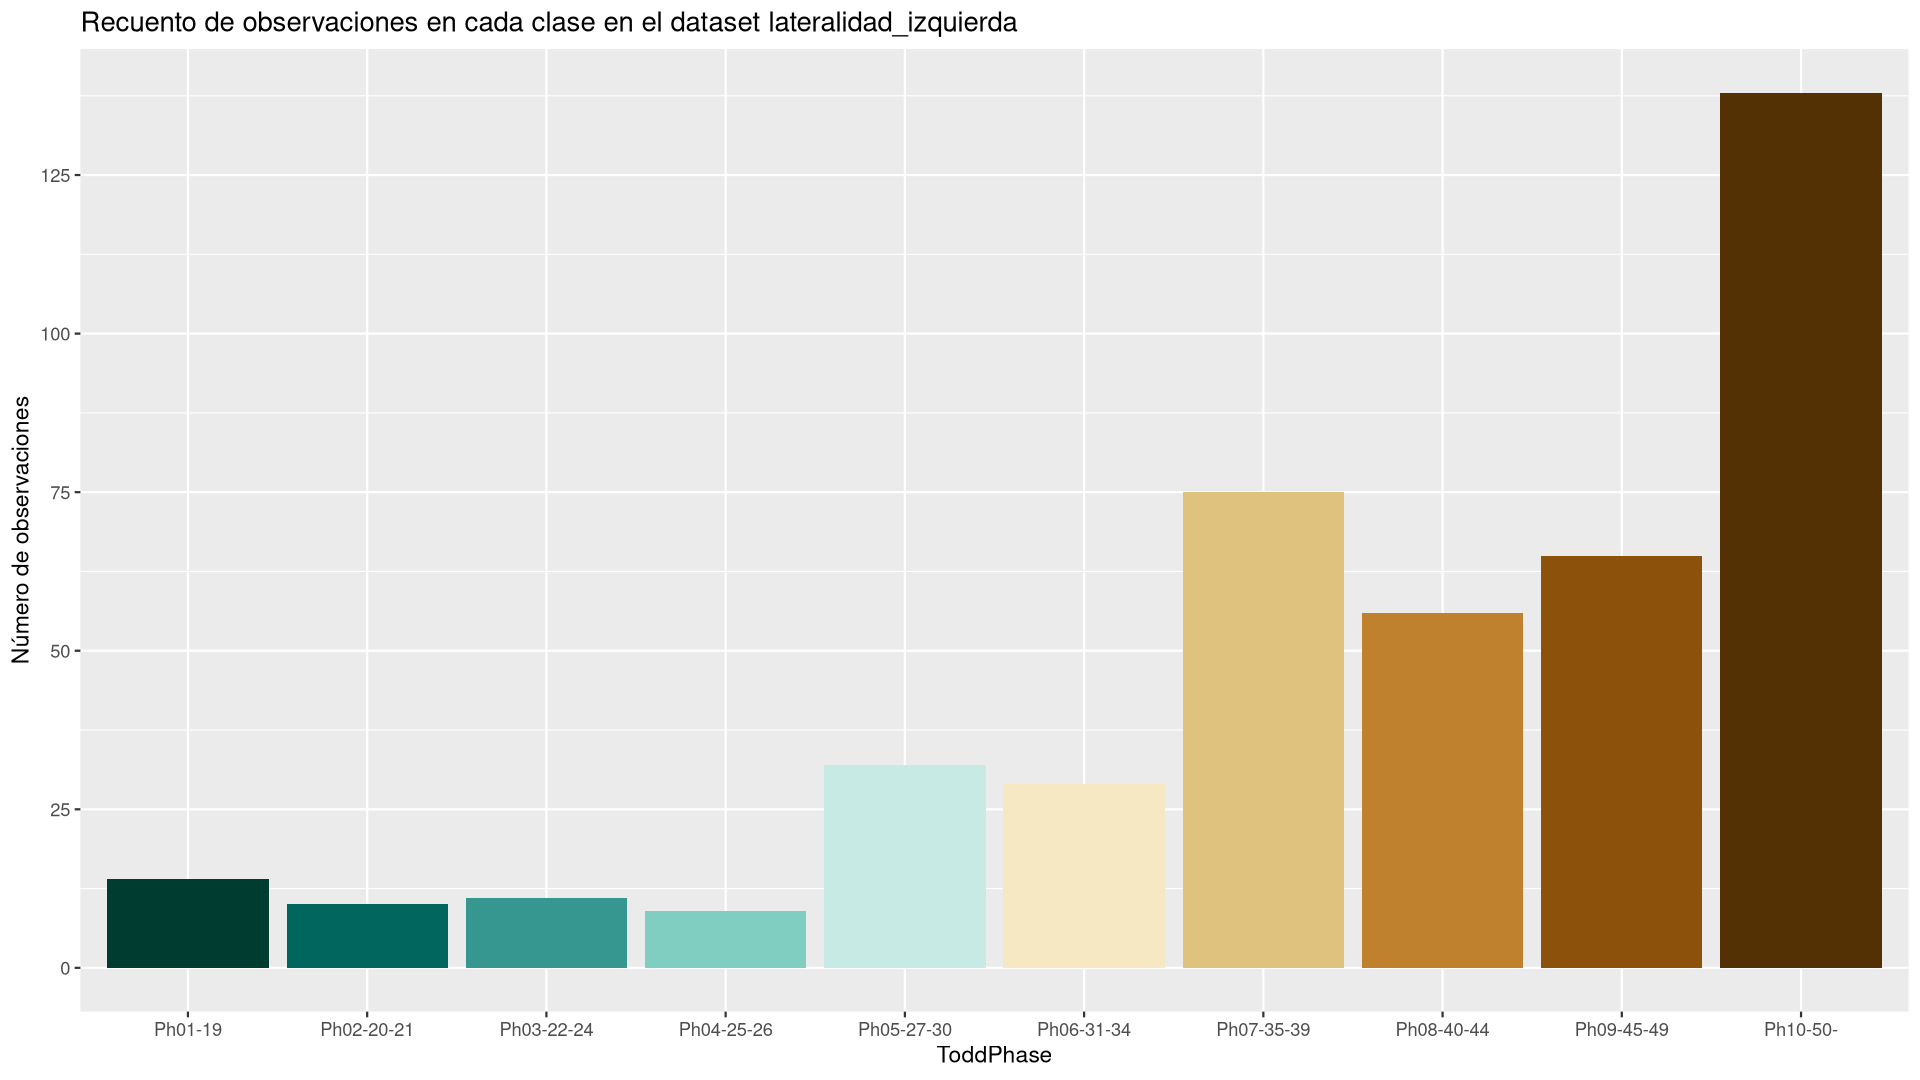
\includegraphics[width = \textwidth]{conjunto_datos/distribucion_clases_lateralidad_izquierda.png}
	\caption{Número de datos por cada fase propuesta por Todd con el conjunto de datos de la lateralidad izquierda.}
	\label{fig:conteo_l0}
\end{figure}

Podemos ver que contamos con una cantidad muy alta de observaciones de las últimas fases en comparación con las primeras fases, en especial de la última fase, de personas de más de cincuenta años.

Debido a que todas las variables del conjunto de datos son categóricas, para este análisis solo podemos observar como se distribuyen los valores de cada predictor para cada fase. Vamos ver cada uno de estos predictores y comentar la información que nos proporcionan.

\begin{figure}[H]
	\centering
	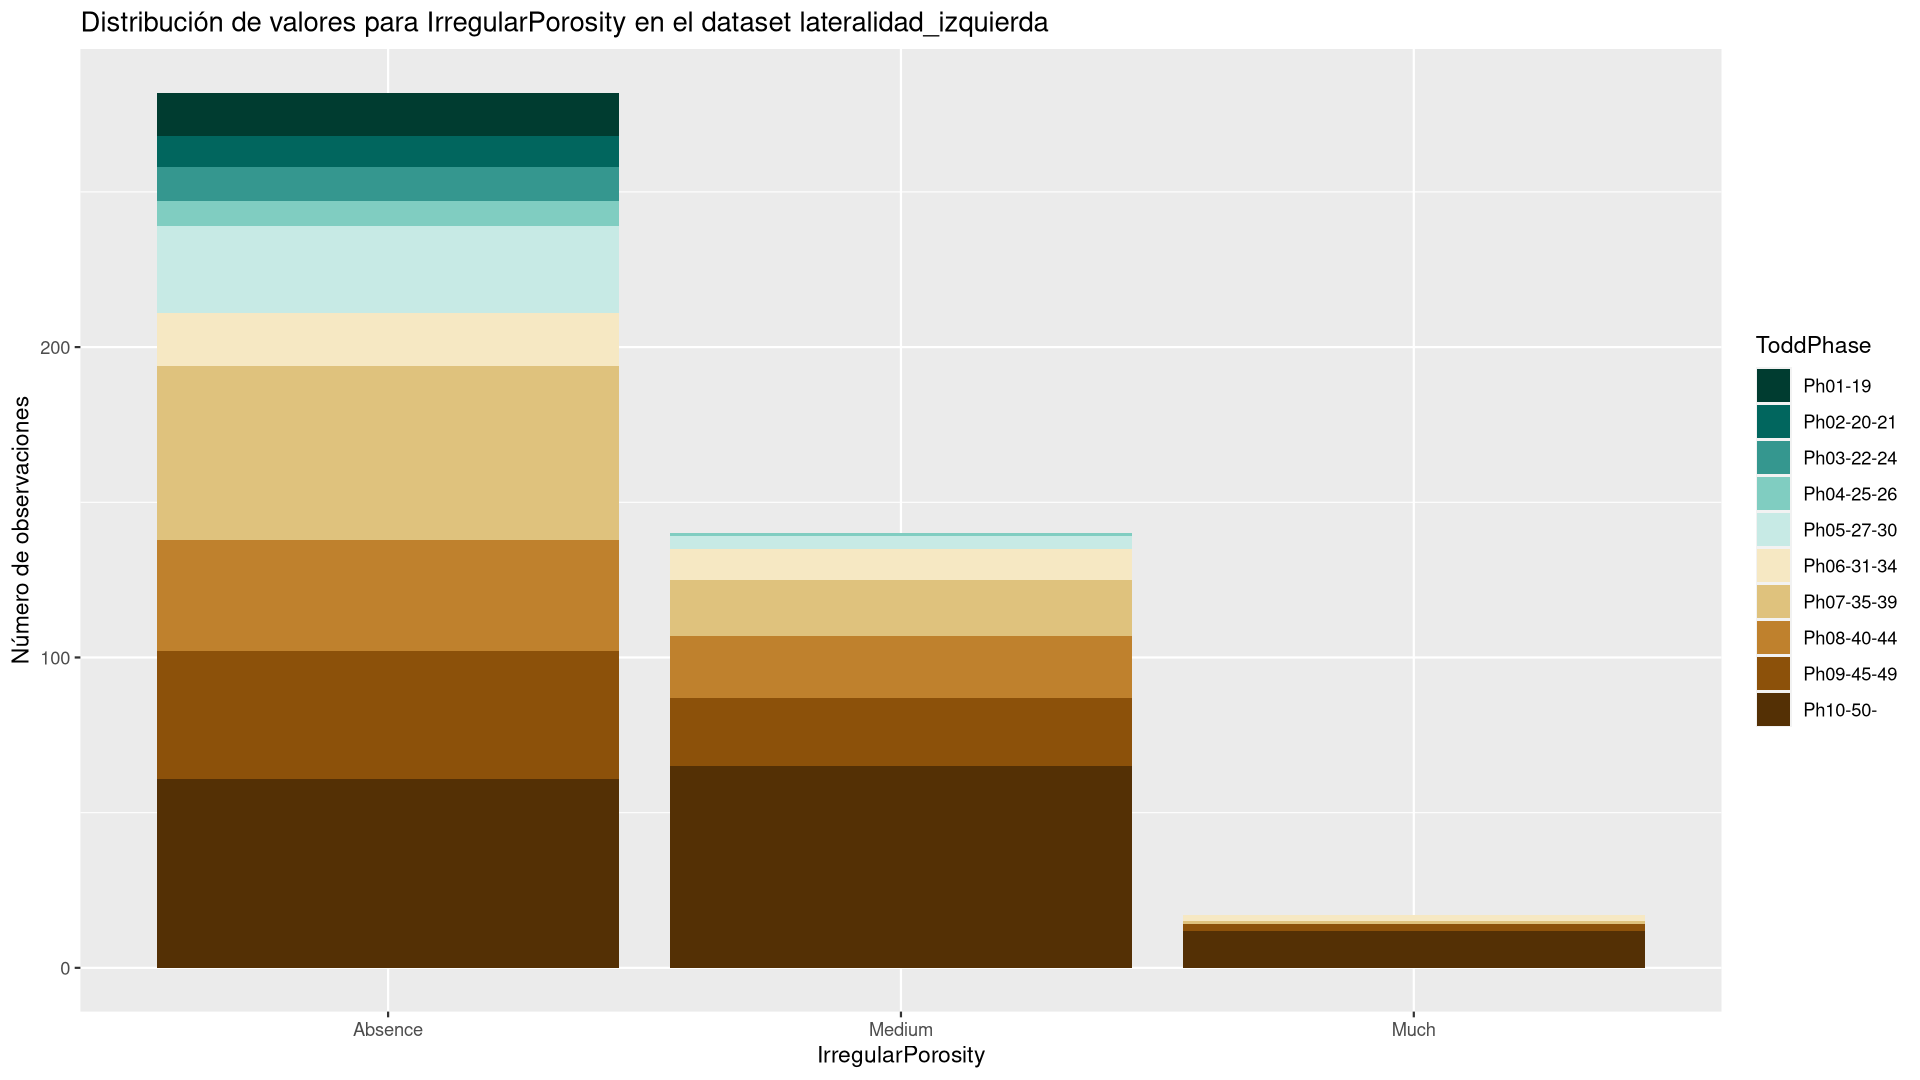
\includegraphics[width = \textwidth]{conjunto_datos/densidad_IrregularPorosity_lateralidad_izquierda.png}
	\caption{Distribución de los valores de IrregularPorosity en el conjunto de datos de la lateralidad izquierda.}
	\label{fig:densidad_IrregularPorosity_lateralidad_izquierda}
\end{figure}

En la figura \ref{fig:densidad_IrregularPorosity_lateralidad_izquierda} podemos observar la distribución de valores de \texttt{IrregularPorosity}. En este vemos como claramente con esta característica podremos clasificar observaciones de clases altas si el valor de esta variable es \texttt{Much}, mientras que con el valor \texttt{Medium} y en especial \texttt{Absence} si hay un mayor solapamiento entre las clases.

Aun así, podemos ver como esta característica tampoco nos aporta gran información para las fases más bajas, donde si se solapa este valor. Vamos a seguir observando el resto de predictores.

\begin{figure}[H]
	\centering
	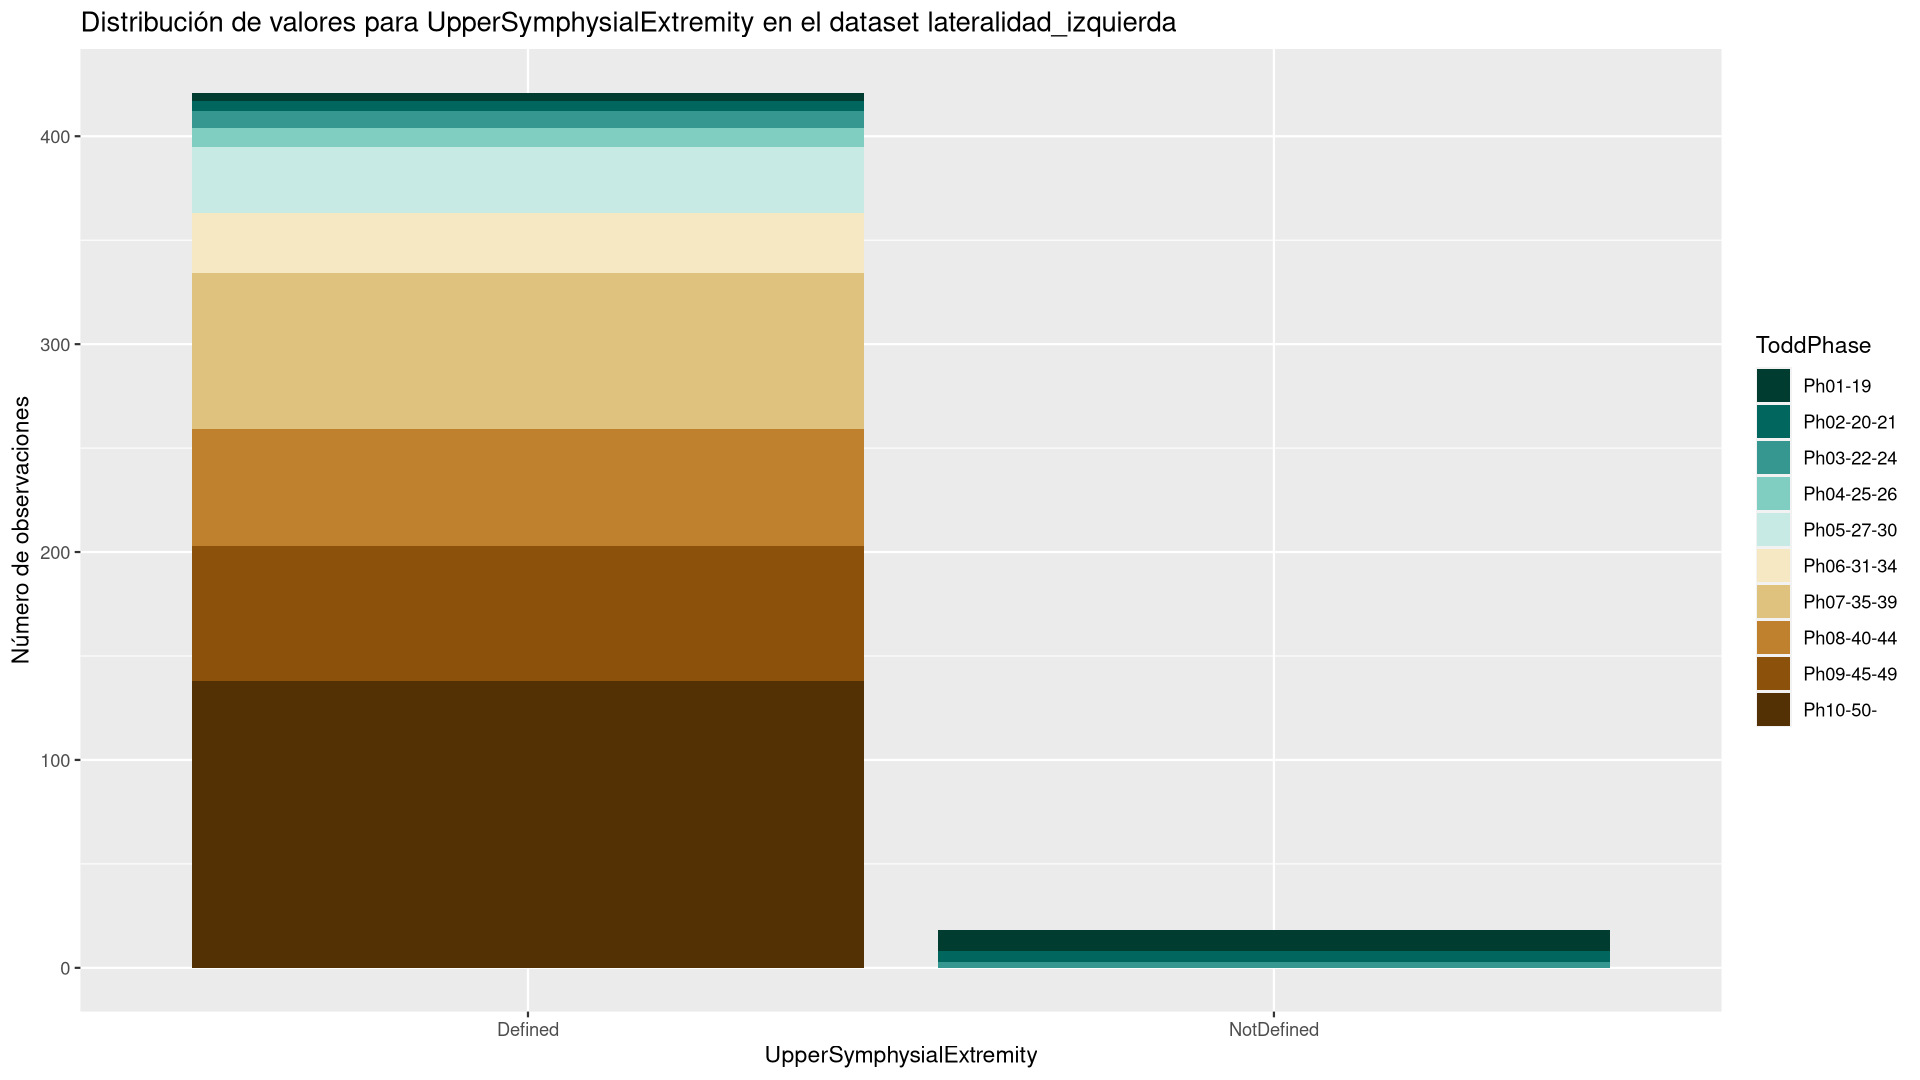
\includegraphics[width = \textwidth]{conjunto_datos/densidad_UpperSymphysialExtremity_lateralidad_izquierda.png}
	\caption{Distribución de los valores de UpperSymphysialExtremity en el conjunto de datos de la lateralidad izquierda.}
	\label{fig:densidad_UpperSymphysialExtremity_lateralidad_izquierda}
\end{figure}

En este caso con \texttt{UpperSymphysialExtremity}, como vemos en la figura \ref{fig:densidad_UpperSymphysialExtremity_lateralidad_izquierda}, ocurre lo contrario que en el caso anterior. Esta característica nos podría servir muy bien para predecir asegurarnos que estamos ante observaciones de fases bajas si toma el valor de \texttt{NotDefined}, sin embargo vemos como las observaciones con este valor siguen existiendo tres posibles clases, por lo que realmente no hemos resuelto por completo estas observaciones, pero si acotado bastante el rango de fases, al ser tres contiguas.

\begin{figure}[H]
	\centering
	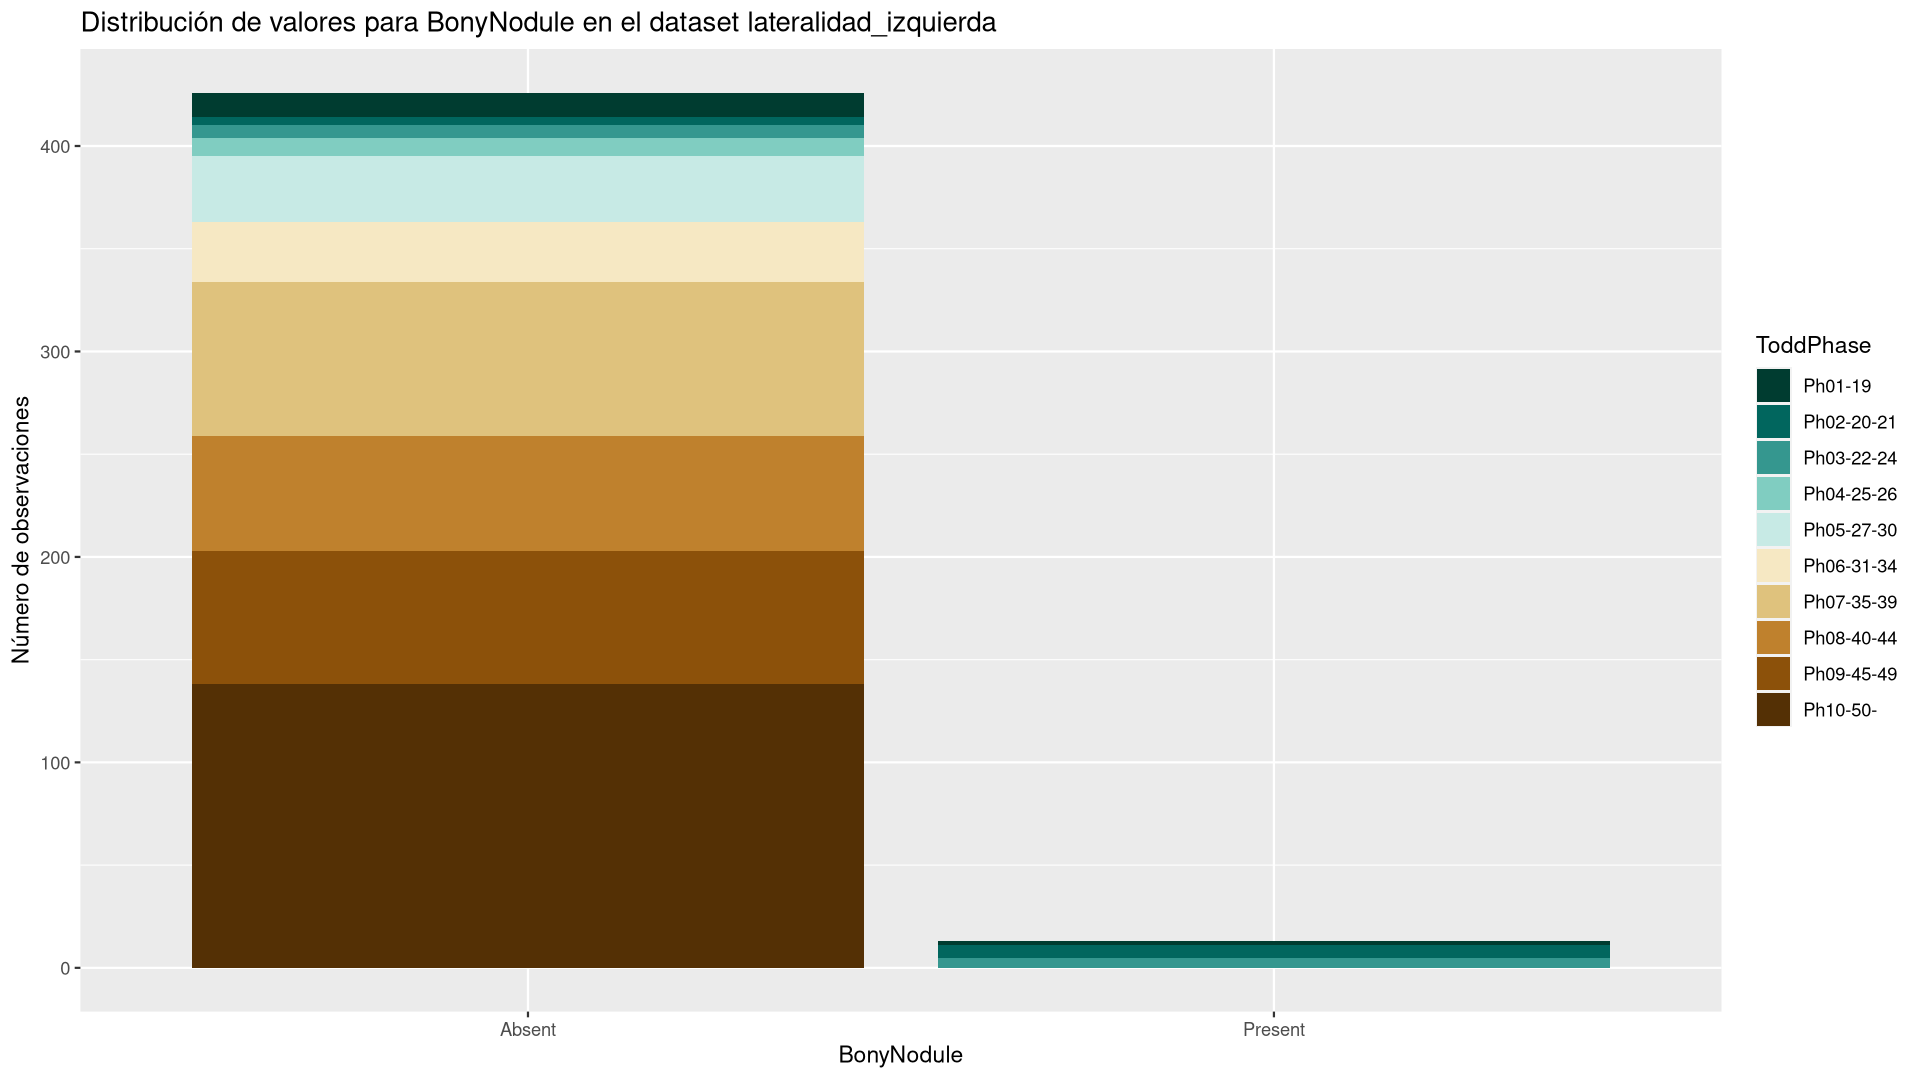
\includegraphics[width = \textwidth]{conjunto_datos/densidad_BonyNodule_lateralidad_izquierda.png}
	\caption{Distribución de los valores de BonyNodule en el conjunto de datos de la lateralidad izquierda.}
	\label{fig:densidad_BonyNodule_lateralidad_izquierda}
\end{figure}

Para la variable \texttt{BonyNodule} ocurre lo mismo que con la variable anterior, \texttt{UpperSymphysialExtremity}. Cuando se toma el valor de \texttt{Present} vemos como todas las observaciones son de fases bajas, aunque sigue existiendo ciertas dudas sobre la fase concreta. Cuando toma el valor de \texttt{Absent} no se puede sacar ninguna conclusión debido a que encontramos valores de todas las clases.

\begin{figure}[H]
	\centering
	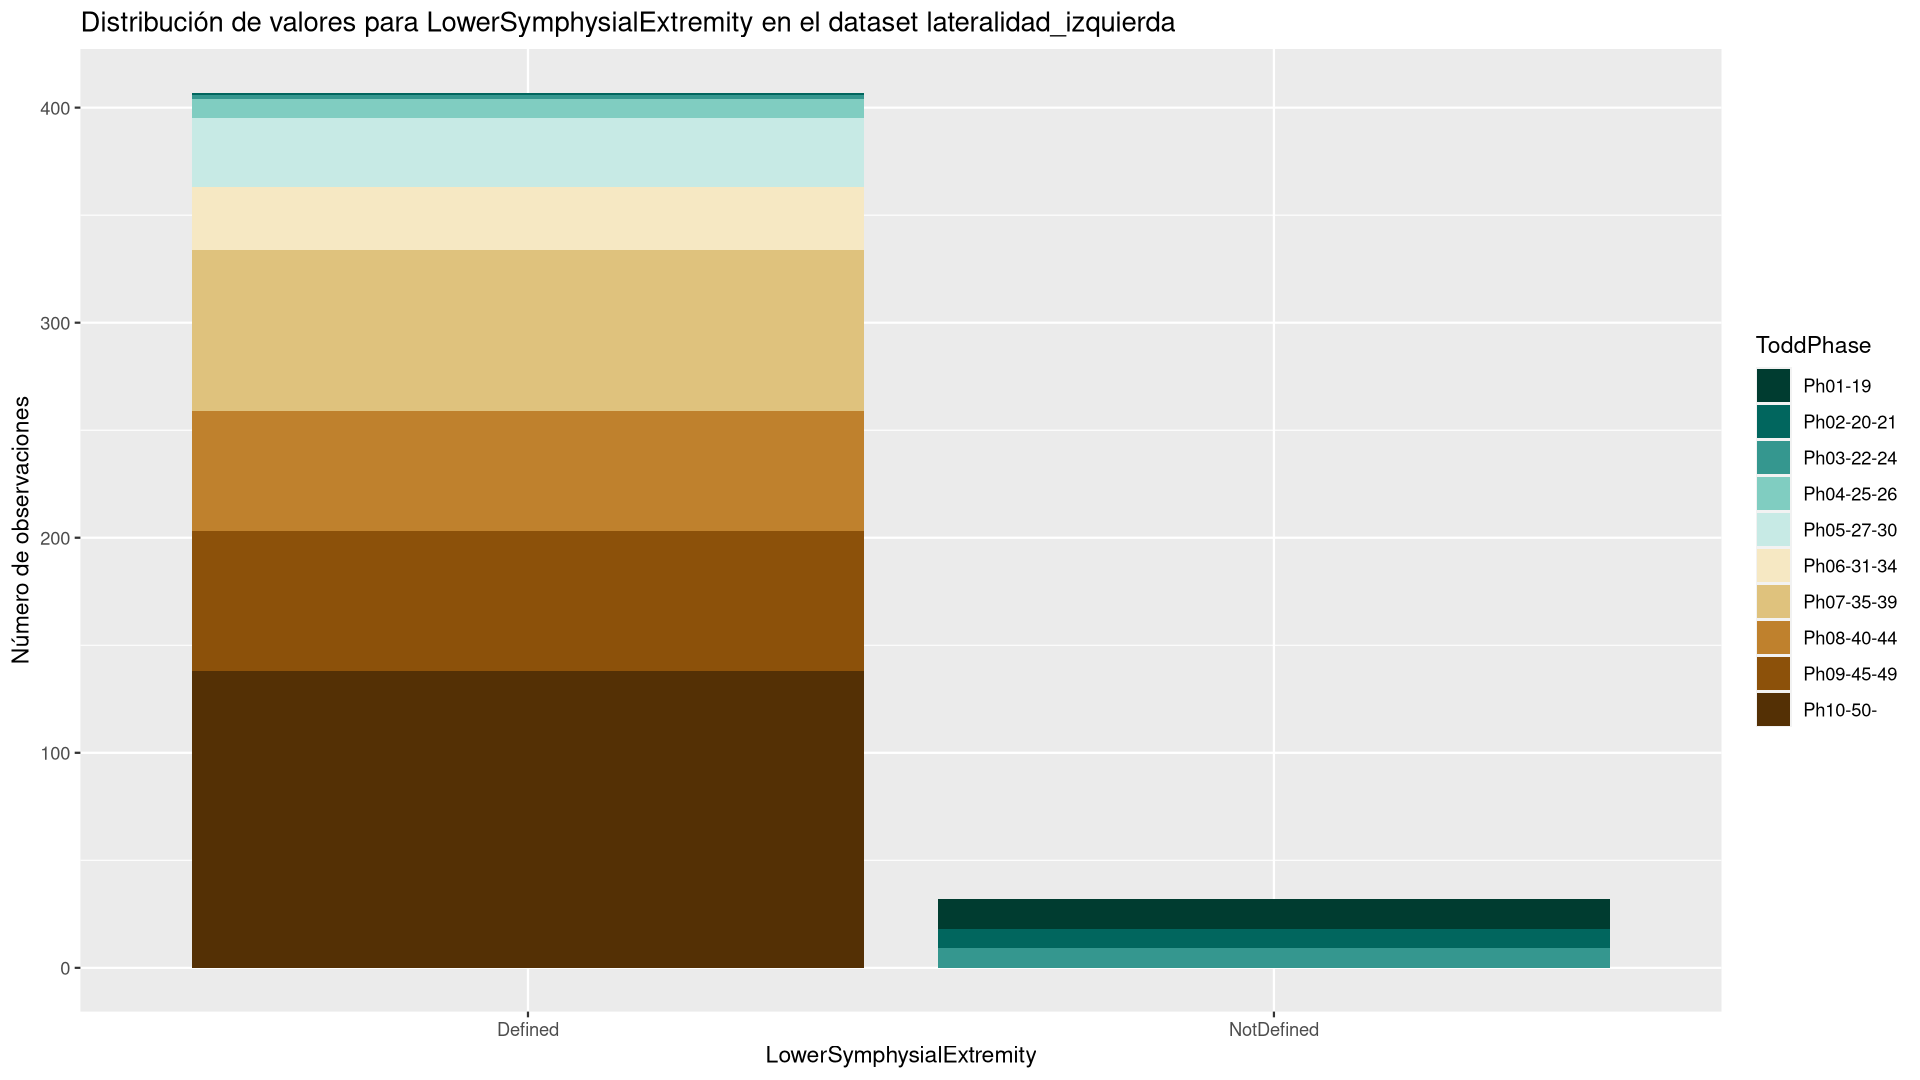
\includegraphics[width = \textwidth]{conjunto_datos/densidad_LowerSymphysialExtremity_lateralidad_izquierda.png}
	\caption{Distribución de los valores de LowerSymphysialExtremity en el conjunto de datos de la lateralidad izquierda.}
	\label{fig:densidad_LowerSymphysialExtremity_lateralidad_izquierda}
\end{figure}

Con \texttt{LowerSymphysialExtremity} se puede observar que ocurre al igual que en casos anteriores, si toma el valor \texttt{NotDefined} podemos ver que se trata de una fase baja, sin embargo, en este caso si que nos llega a aportar algo más de información. En los casos anteriores, aunque un valor nos discriminaba muy bien si era de una fase temprana o no, el valor contrario seguía teniendo valores de todas las clases, es decir, si por ejemplo \texttt{BonyNodule} toma el valor \texttt{Present}, sabemos que se trata de una fase temprana, sin embargo si toma el valor \texttt{Absent} no podemos decir nada, porque podría ser de cualquier fase, sin embargo, con \texttt{LowerSymphysialExtremity} podemos ver claramente como si es \texttt{NotDefined} será de una clase baja, pero si es \texttt{Defined} podemos concluir que, al menos de la primera fase no será esta observación, ya que no encontramos observaciones de esta fase, y muy pocas de la fase dos y tres.

\begin{figure}[H]
	\centering
	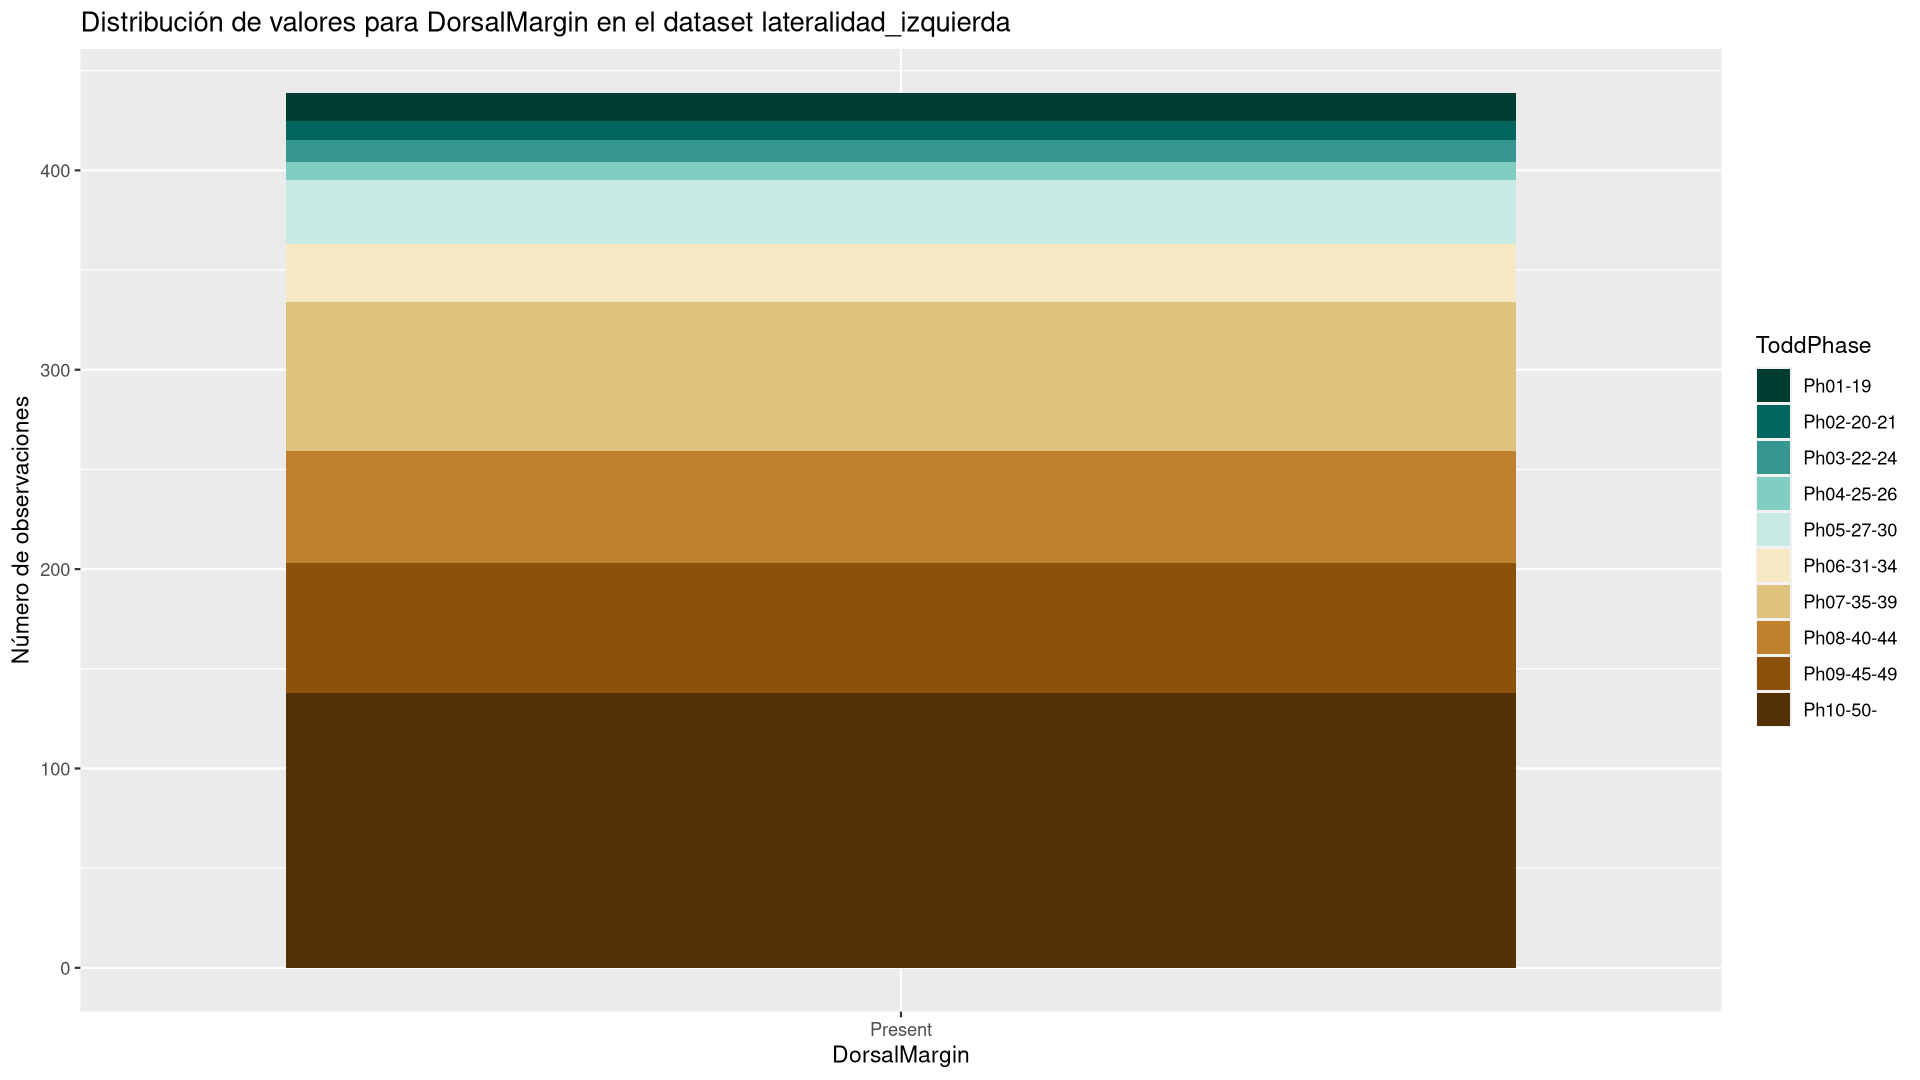
\includegraphics[width = \textwidth]{conjunto_datos/densidad_DorsalMargin_lateralidad_izquierda.png}
	\caption{Distribución de los valores de DorsalMargin en el conjunto de datos de la lateralidad izquierda.}
	\label{fig:densidad_DorsalMargin_izquierda}
\end{figure}

En este caso \texttt{DorsalMargin} vemos como no aporta información alguna, ya que solo toma un valor independientemente de la fase de edad. Si esto sigue ocurriendo en la lateralidad derecha (y por lo tanto en el conjunto completo, al ser la unión de este conjunto y la lateralidad derecha), podemos eliminar esta característica a la hora de entrenar el modelo ya que no aportaría información alguna al modelo.

\begin{figure}[H]
	\centering
	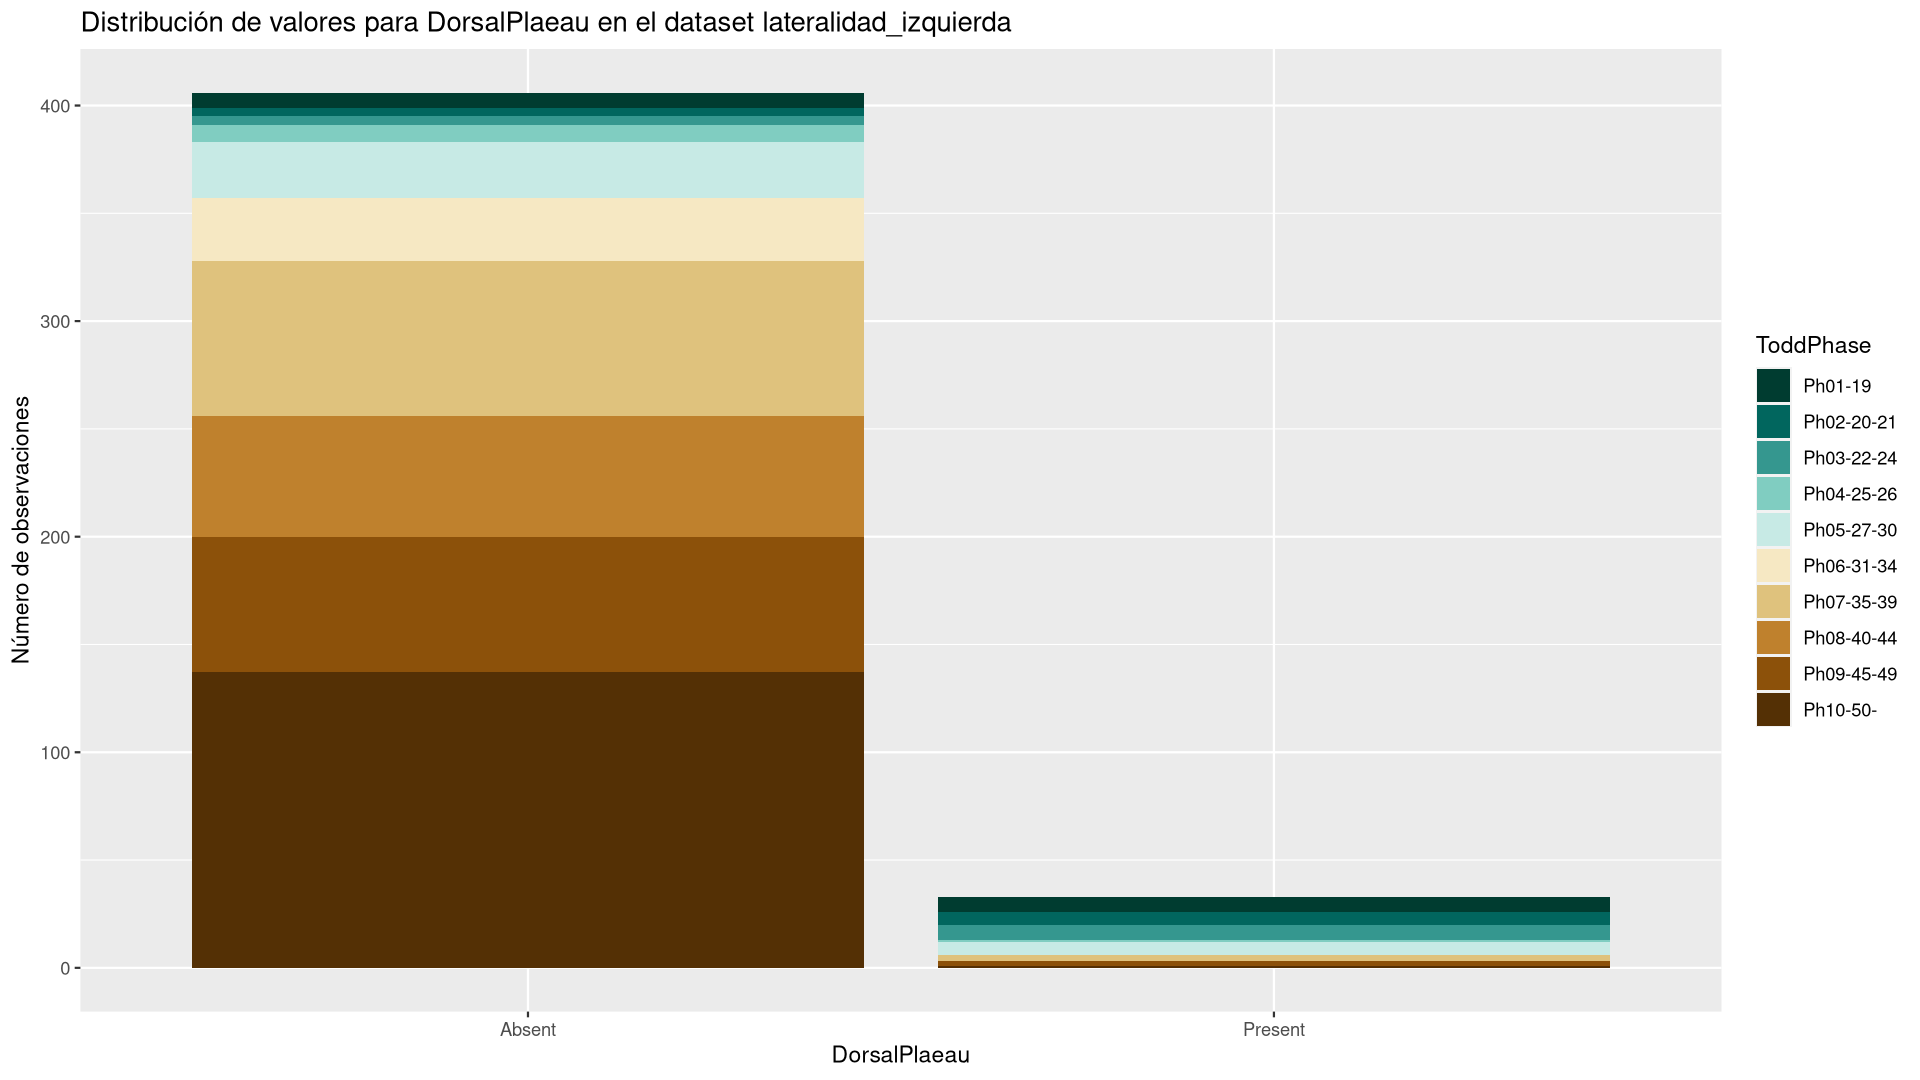
\includegraphics[width = \textwidth]{conjunto_datos/densidad_DorsalPlaeau_lateralidad_izquierda.png}
	\caption{Distribución de los valores de DorsalPlaeau en el conjunto de datos de la lateralidad izquierda.}
	\label{fig:densidad_DorsalPlaeau_izquierda}
\end{figure}

Para los valores de \texttt{DorsalPlaeau} vemos como si que toma distintos valores, sin embargo estos no nos aportan mucha información, ya que tanto para \texttt{Absent} como para \texttt{Present} contamos con observaciones de todo tipo de fases, tanto altas como bajas, luego a priori no podemos saber si este predictor será de gran utilidad.

\begin{figure}[H]
	\centering
	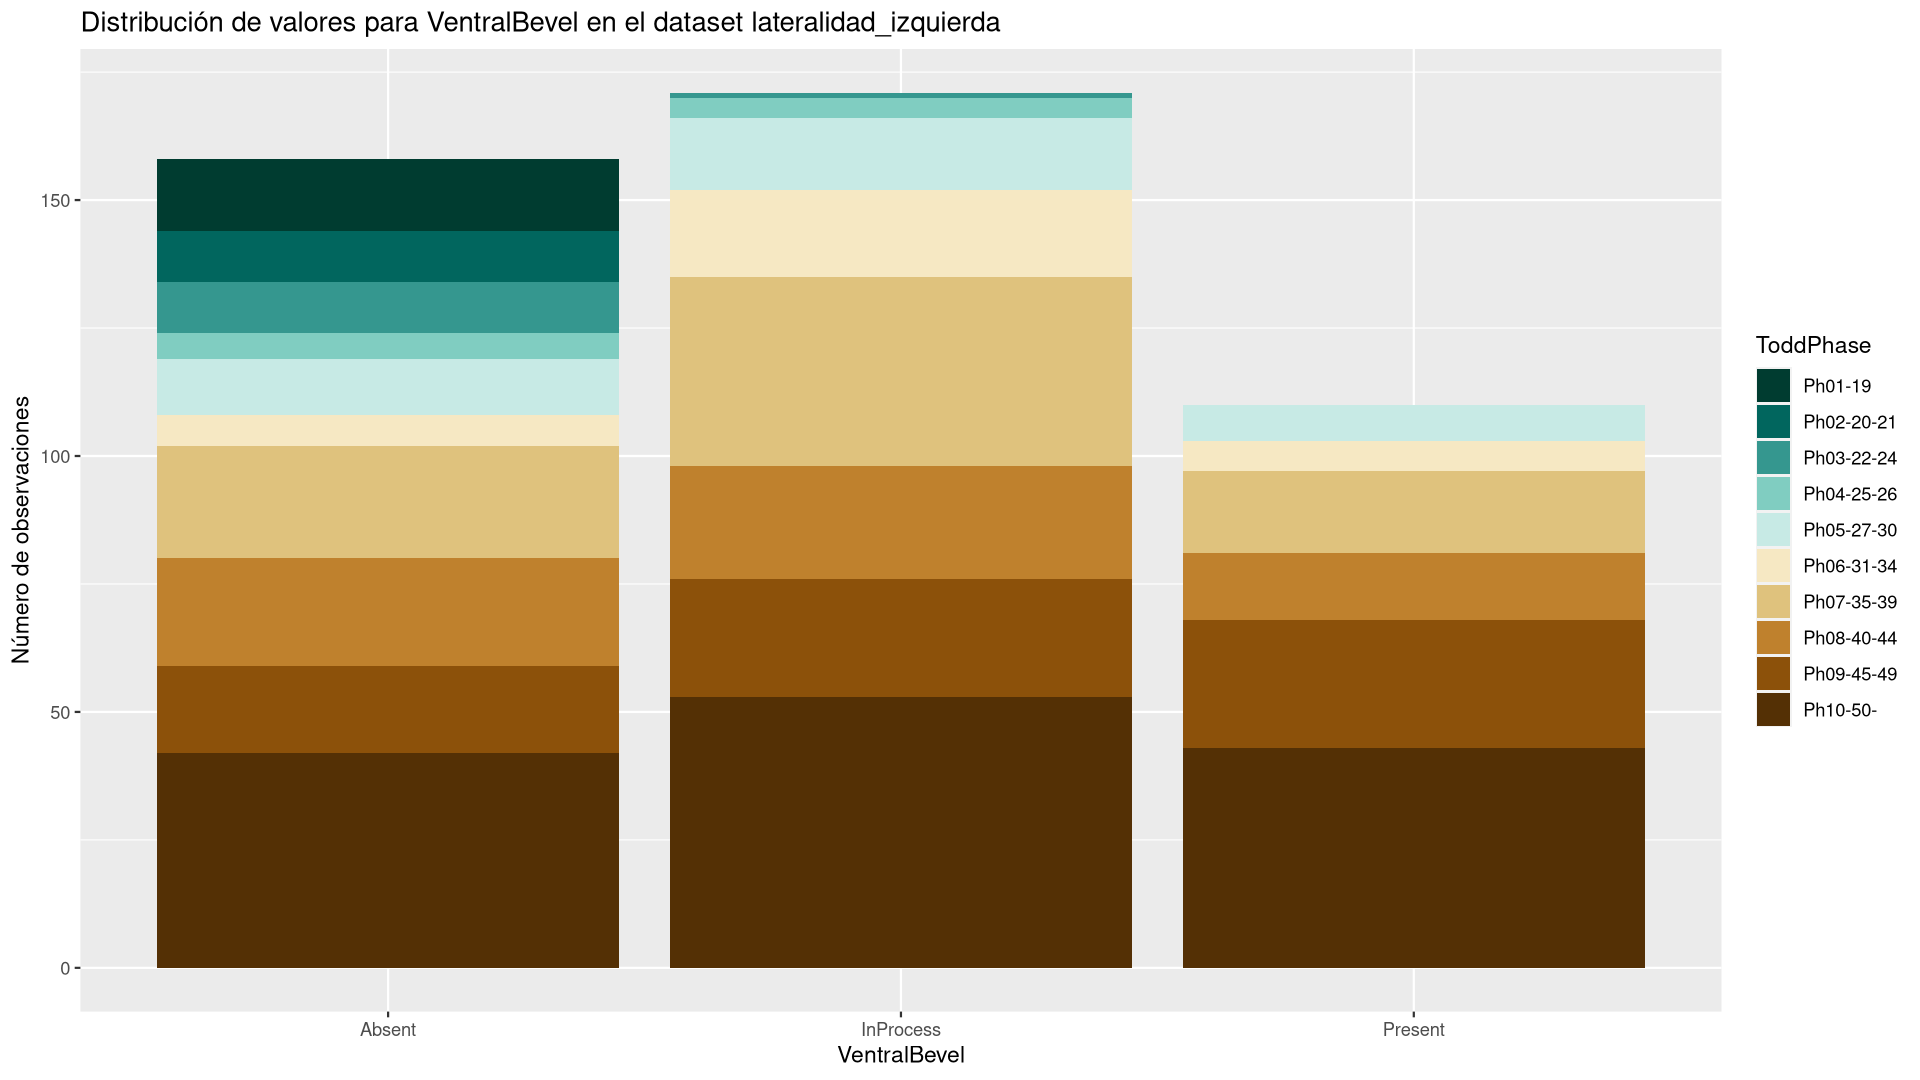
\includegraphics[width = \textwidth]{conjunto_datos/densidad_VentralBevel_lateralidad_izquierda.png}
	\caption{Distribución de los valores de VentralBevel en el conjunto de datos de la lateralidad izquierda.}
	\label{fig:densidad_VentralBevel_izquierda}
\end{figure}

Aunque con \texttt{VentralBevel} vemos como para los distintos valores tenemos una gran variedad de clases, si que podemos sacar algunas conclusiones de este gráfico, voy a comentarlas según cada valor que puede tomar esta variable. Empezando con \texttt{Absent}, podemos ver como no podemos sacar ninguna conclusión, al tener observaciones de todo tipo de fases. Con \texttt{InProcess} se observa que aunque sigue existiendo observaciones de casi todas las fases, no tenemos de la fase uno, y las observaciones de la fase dos sin mínimas. Esto sumado a que con valores de \texttt{Present} solo se tienen observaciones de fases mayores a la fase cinco, este predictor nos puede ser de utilidad para acotar el resultado, ya que gran cantidad de observaciones toman el valor de \texttt{Present}, y con esto sabemos que son de una fase más alta y aunque siga existiendo variedad de clases, hemos conseguido acotarla.


\begin{figure}[H]
	\centering
	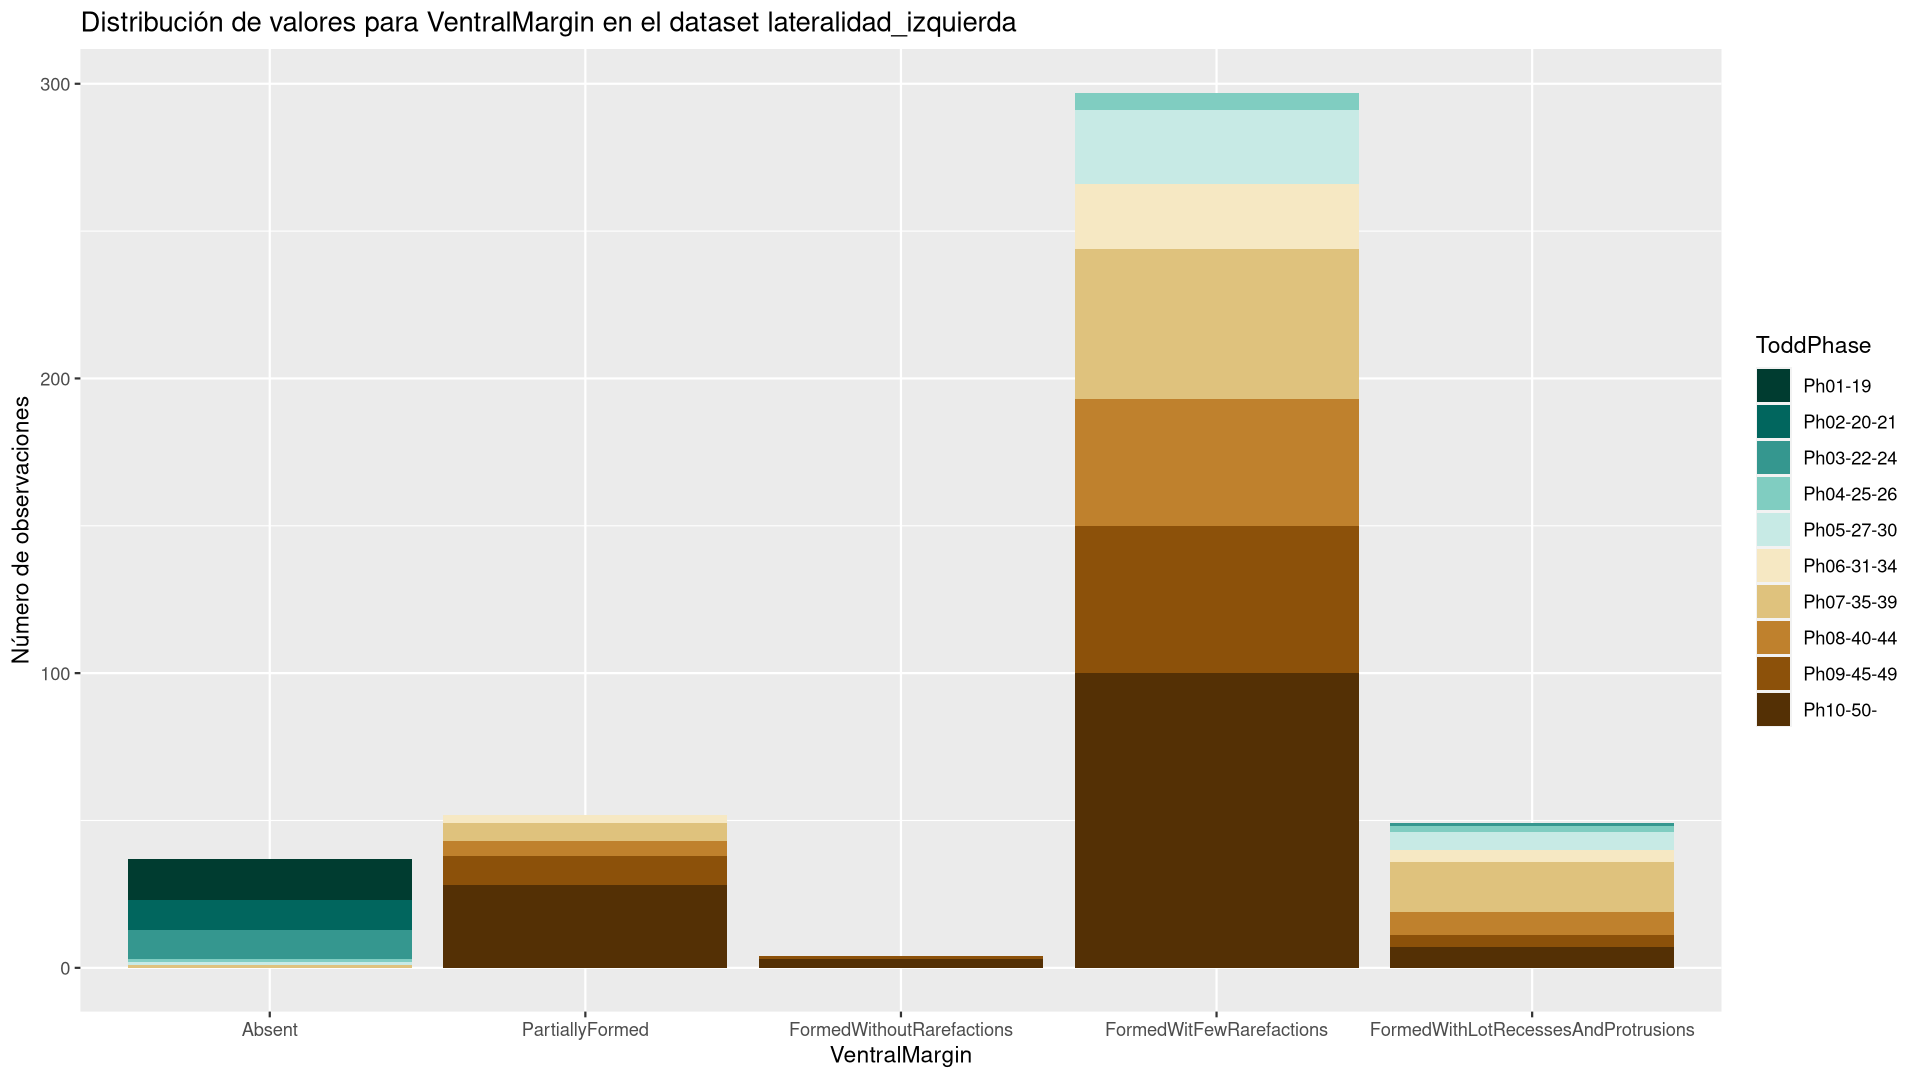
\includegraphics[width = \textwidth]{conjunto_datos/densidad_VentralMargin_lateralidad_izquierda.png}
	\caption{Distribución de los valores de VentralMargin en el conjunto de datos de la lateralidad izquierda.}
	\label{fig:densidad_VentralMargin_izquierda}
\end{figure}

Para \texttt{VentralMargin} vemos como claramente si toma el valor de \texttt{Absent} nos indica que la observación de una fase temprana, si toma el valor de \texttt{PartiallyFormed} estamos ante una observación de una fase mayor o igual a la sexta, y si toma el valor de \texttt{FormedWithoutRarefactions} se trata de una observación de la última fase. Con respecto al resto de valores, \texttt{FormedWithFewRarefactions} sigue teniendo una cantidad alta de fases, pero nos puede dar la información de que la observación no es de las tres fases más tempranas, mientras que \texttt{FormedWithLotRecessesAndProtrusions} no nos da ninguna información de la clase debido al solape de fases que existen.

\newpage

\subsubsection{Análisis de la lateralidad derecha}

Este conjunto de datos cuenta con 453 muestras. Al igual que con la lateralidad izquierda, vamos a ver de forma gráfica como se distribuyen los datos según las fases propuestas por Todd. Debido a la similitud de con la lateralidad izquierda, si las conclusiones obtenidas son semejantes a las obtenidas anteriormente para cada predictor no se comentarán por evitar repetirse:

\begin{figure}[H]
	\centering
	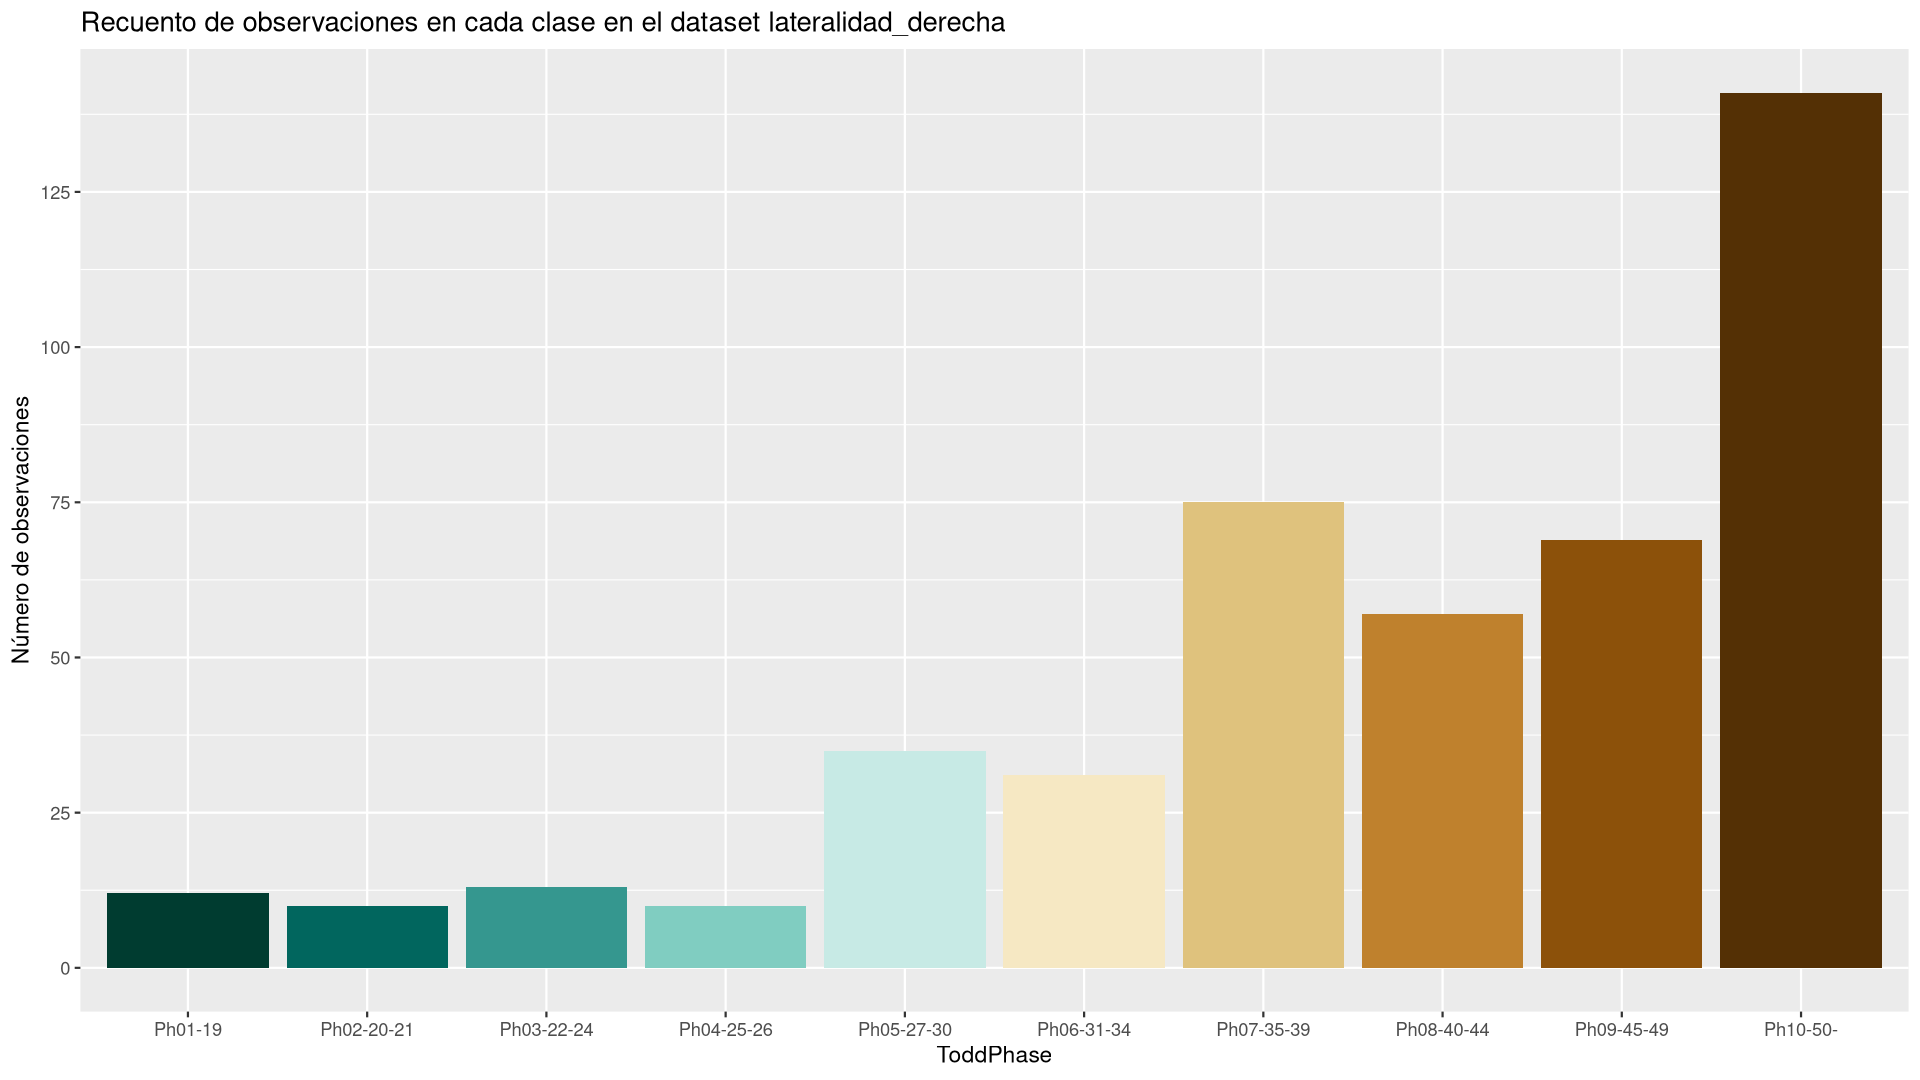
\includegraphics[width = \textwidth]{conjunto_datos/distribucion_clases_lateralidad_derecha.png}
	\caption{Número de datos por cada fase propuesta por Todd con el conjunto de datos de la lateralidad derecha.}
	\label{fig:conteo_l1}
\end{figure}


\begin{figure}[H]
	\centering
	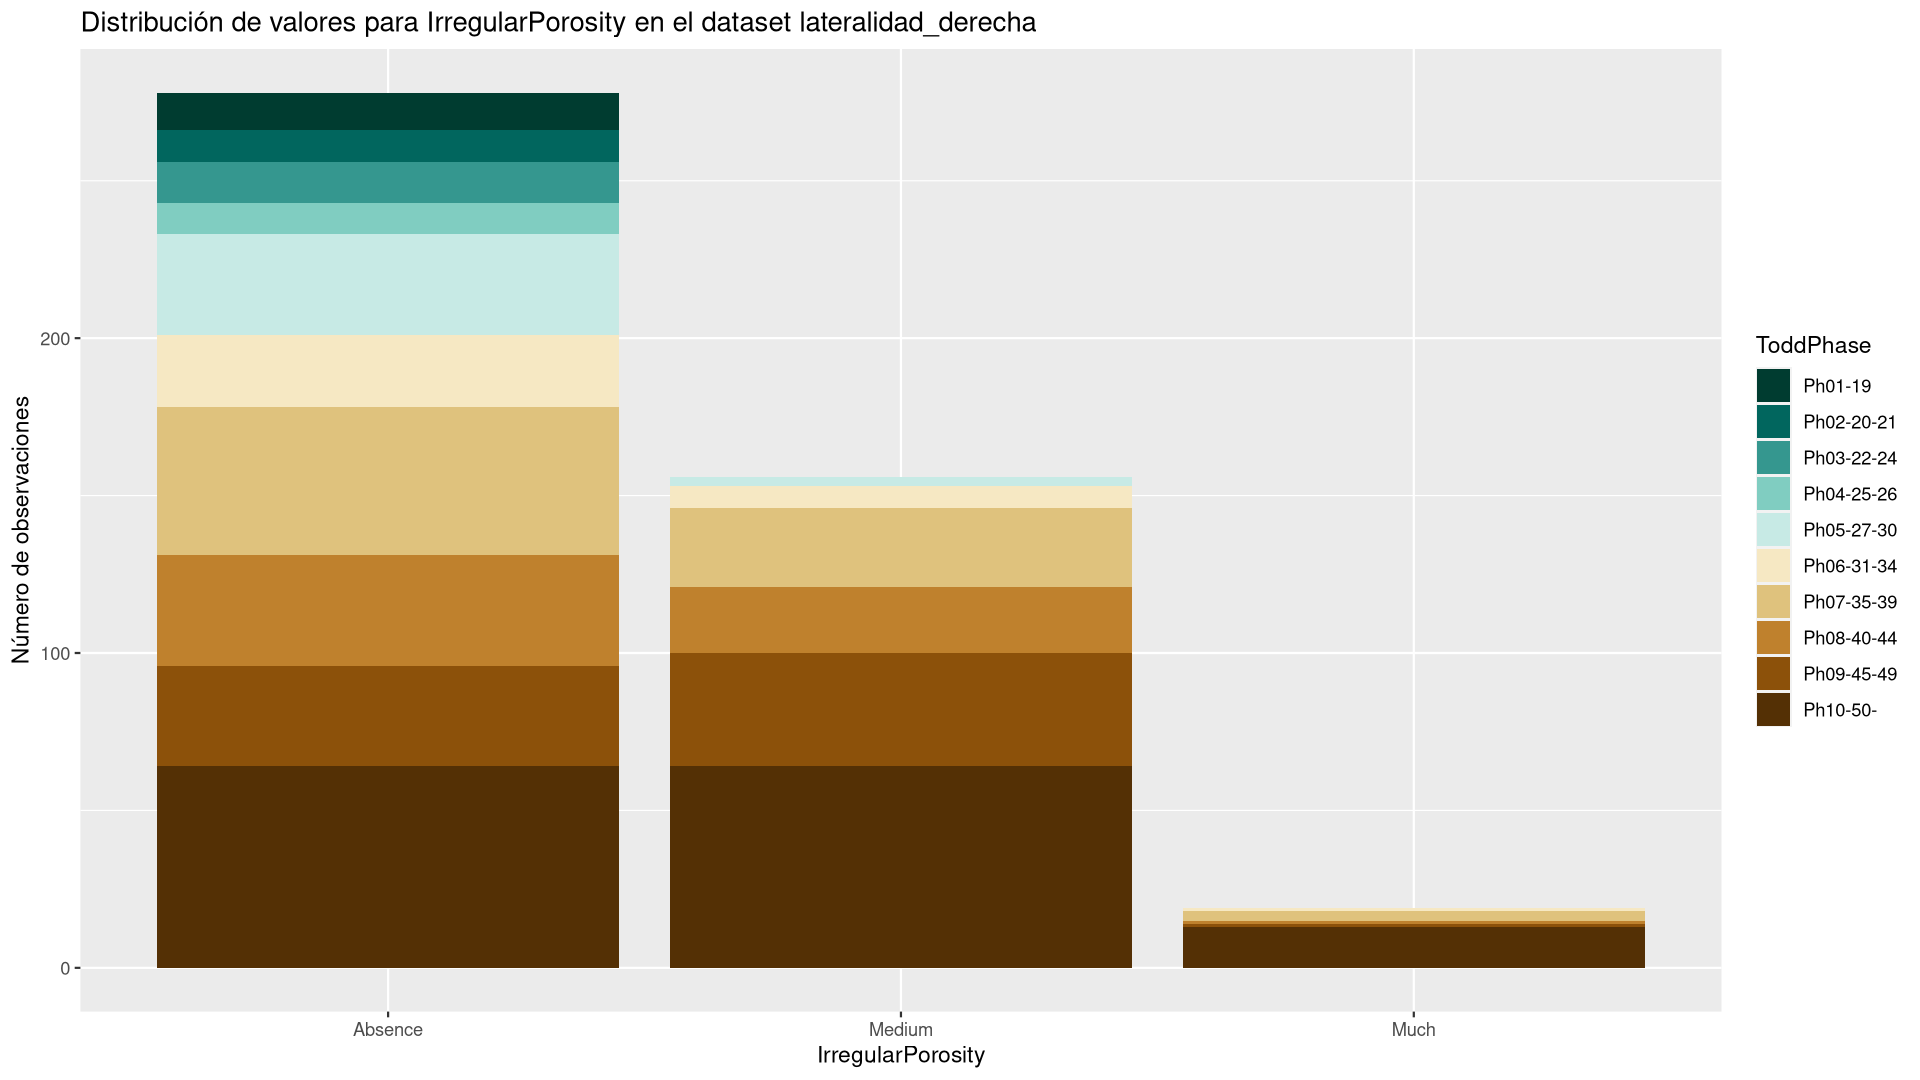
\includegraphics[width = \textwidth]{conjunto_datos/densidad_IrregularPorosity_lateralidad_derecha.png}
	\caption{Distribución de los valores de IrregularPorosity en el conjunto de datos de la lateralidad derecha.}
	\label{fig:densidad_IrregularPorosity_lateralidad_derecha}
\end{figure}

\begin{figure}[H]
	\centering
	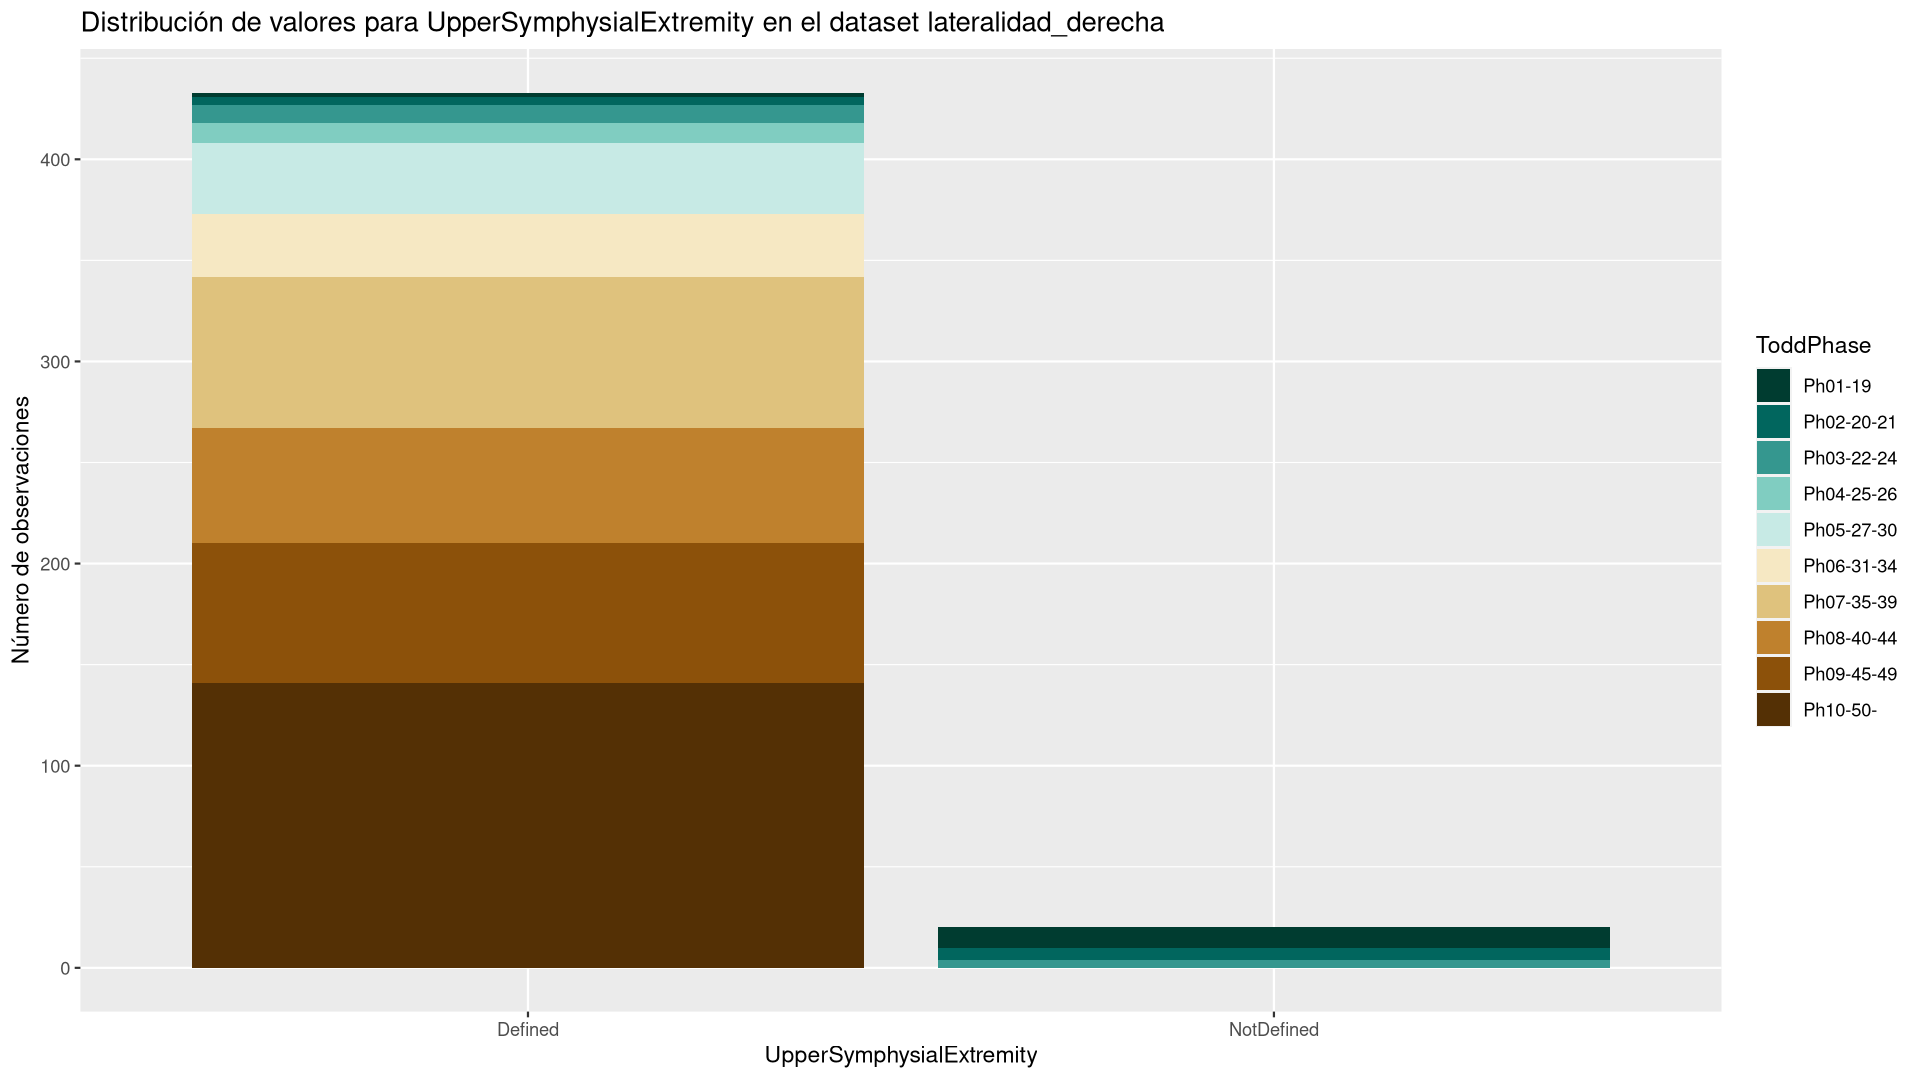
\includegraphics[width = \textwidth]{conjunto_datos/densidad_UpperSymphysialExtremity_lateralidad_derecha.png}
	\caption{Distribución de los valores de UpperSymphysialExtremity en el conjunto de datos de la lateralidad derecha.}
	\label{fig:densidad_UpperSymphysialExtremity_lateralidad_derecha}
\end{figure}


\begin{figure}[H]
	\centering
	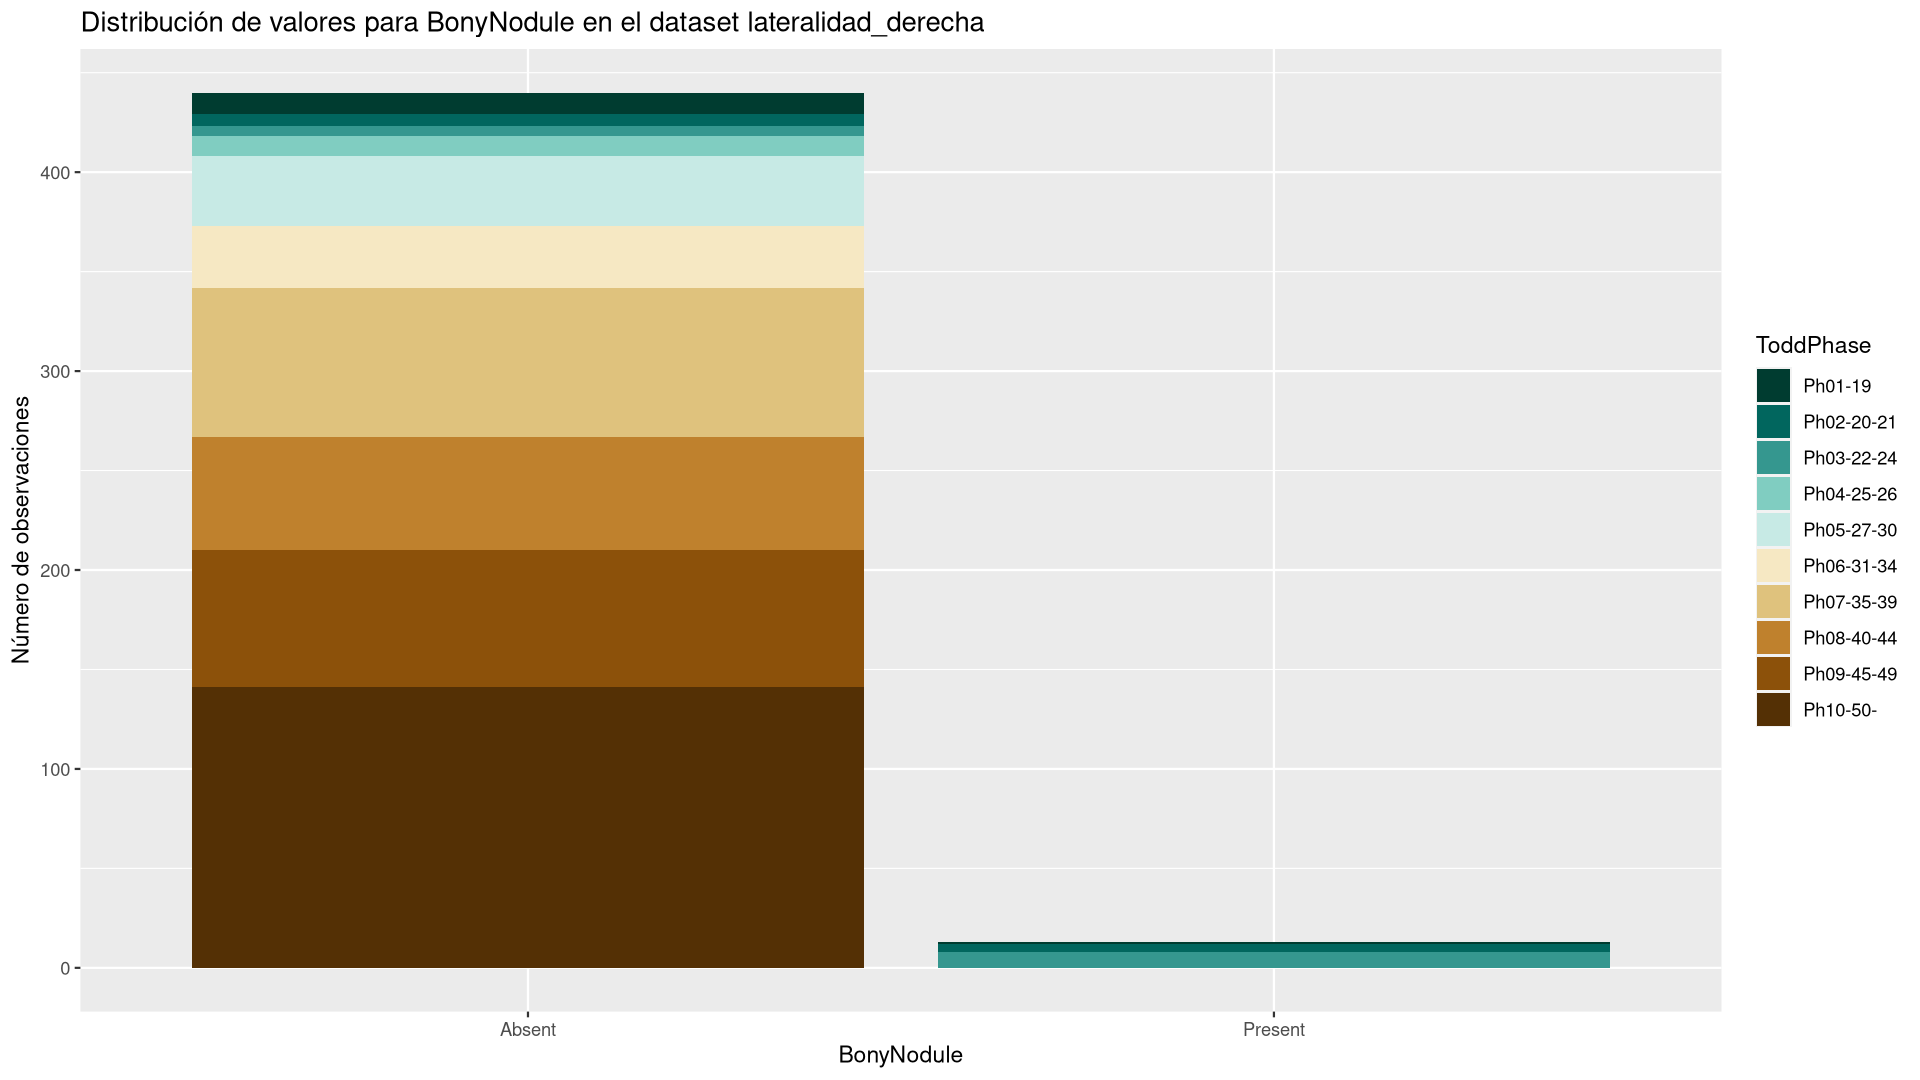
\includegraphics[width = \textwidth]{conjunto_datos/densidad_BonyNodule_lateralidad_derecha.png}
	\caption{Distribución de los valores de BonyNodule en el conjunto de datos de la lateralidad derecha.}
	\label{fig:densidad_BonyNodule_lateralidad_derecha}
\end{figure}



\begin{figure}[H]
	\centering
	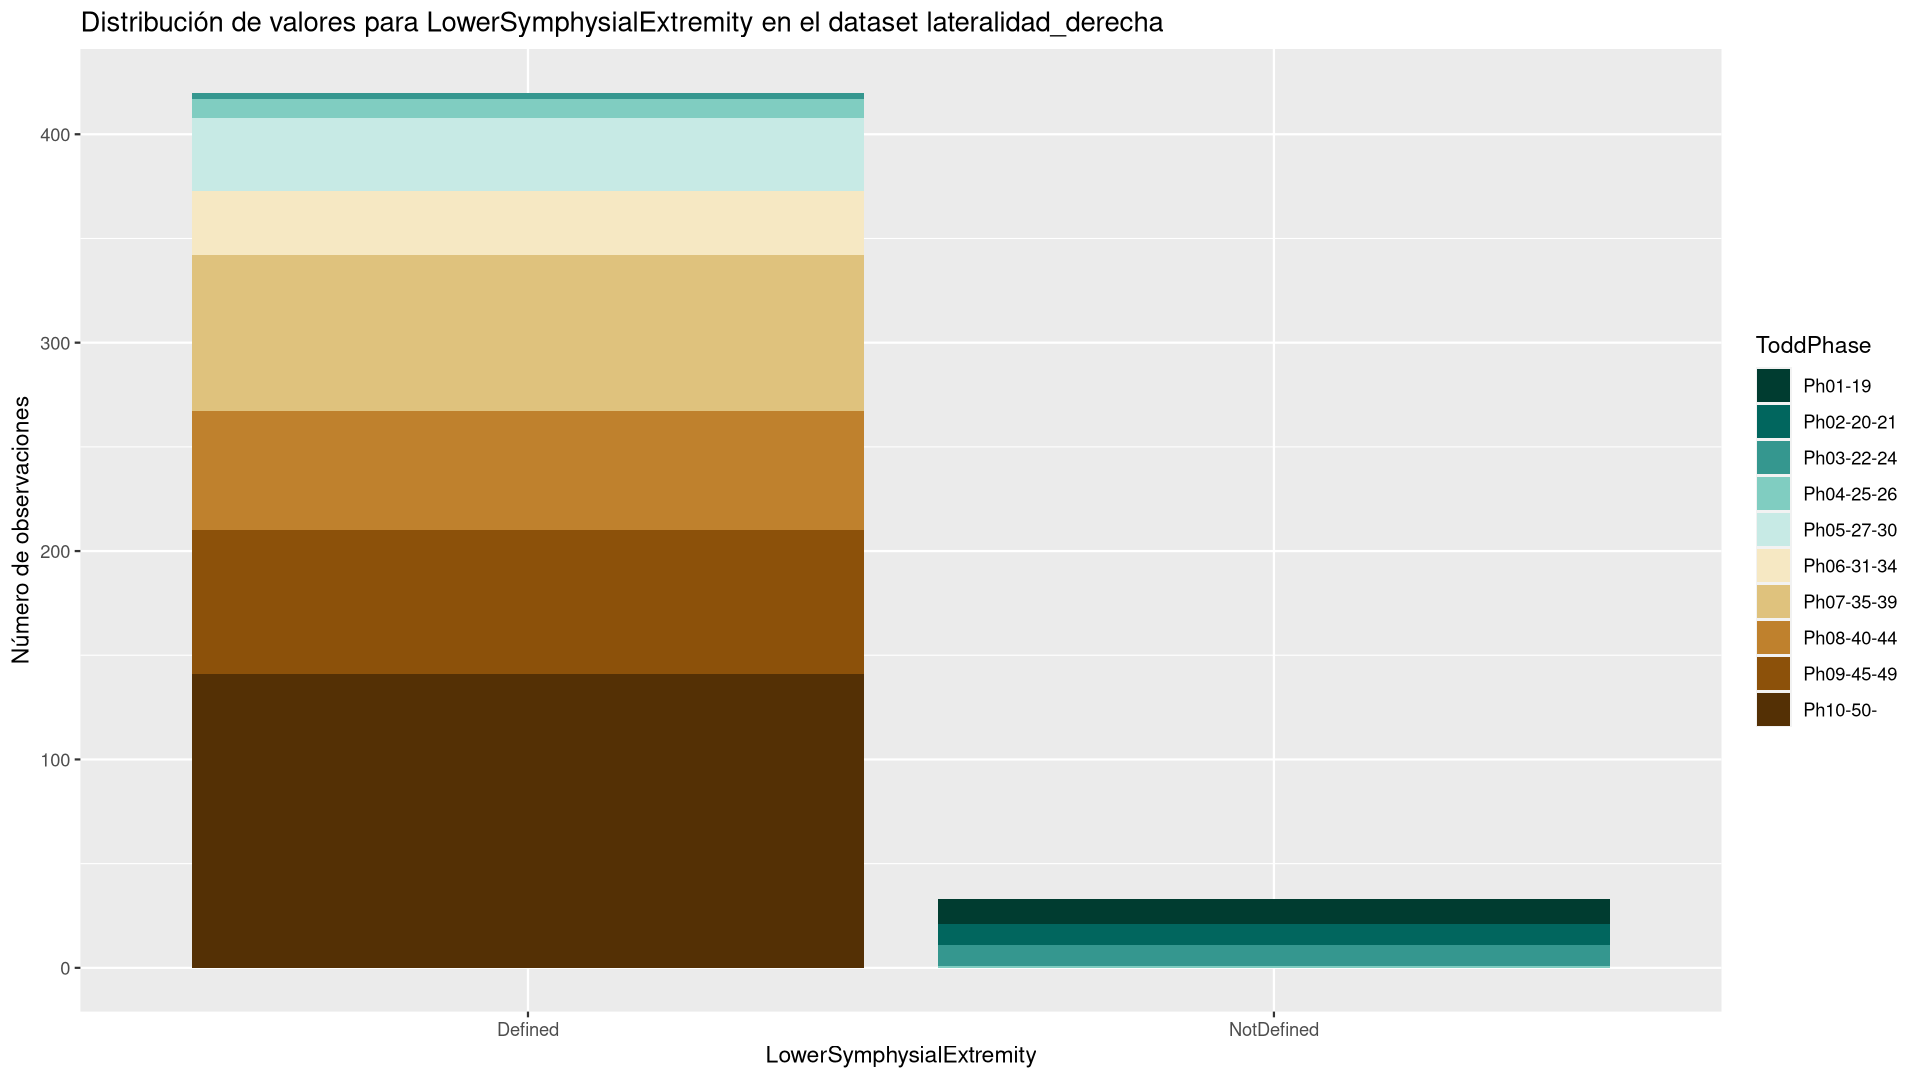
\includegraphics[width = \textwidth]{conjunto_datos/densidad_LowerSymphysialExtremity_lateralidad_derecha.png}
	\caption{Distribución de los valores de LowerSymphysialExtremity en el conjunto de datos de la lateralidad derecha.}
	\label{fig:densidad_LowerSymphysialExtremity_derecha}
\end{figure}


\begin{figure}[H]
	\centering
	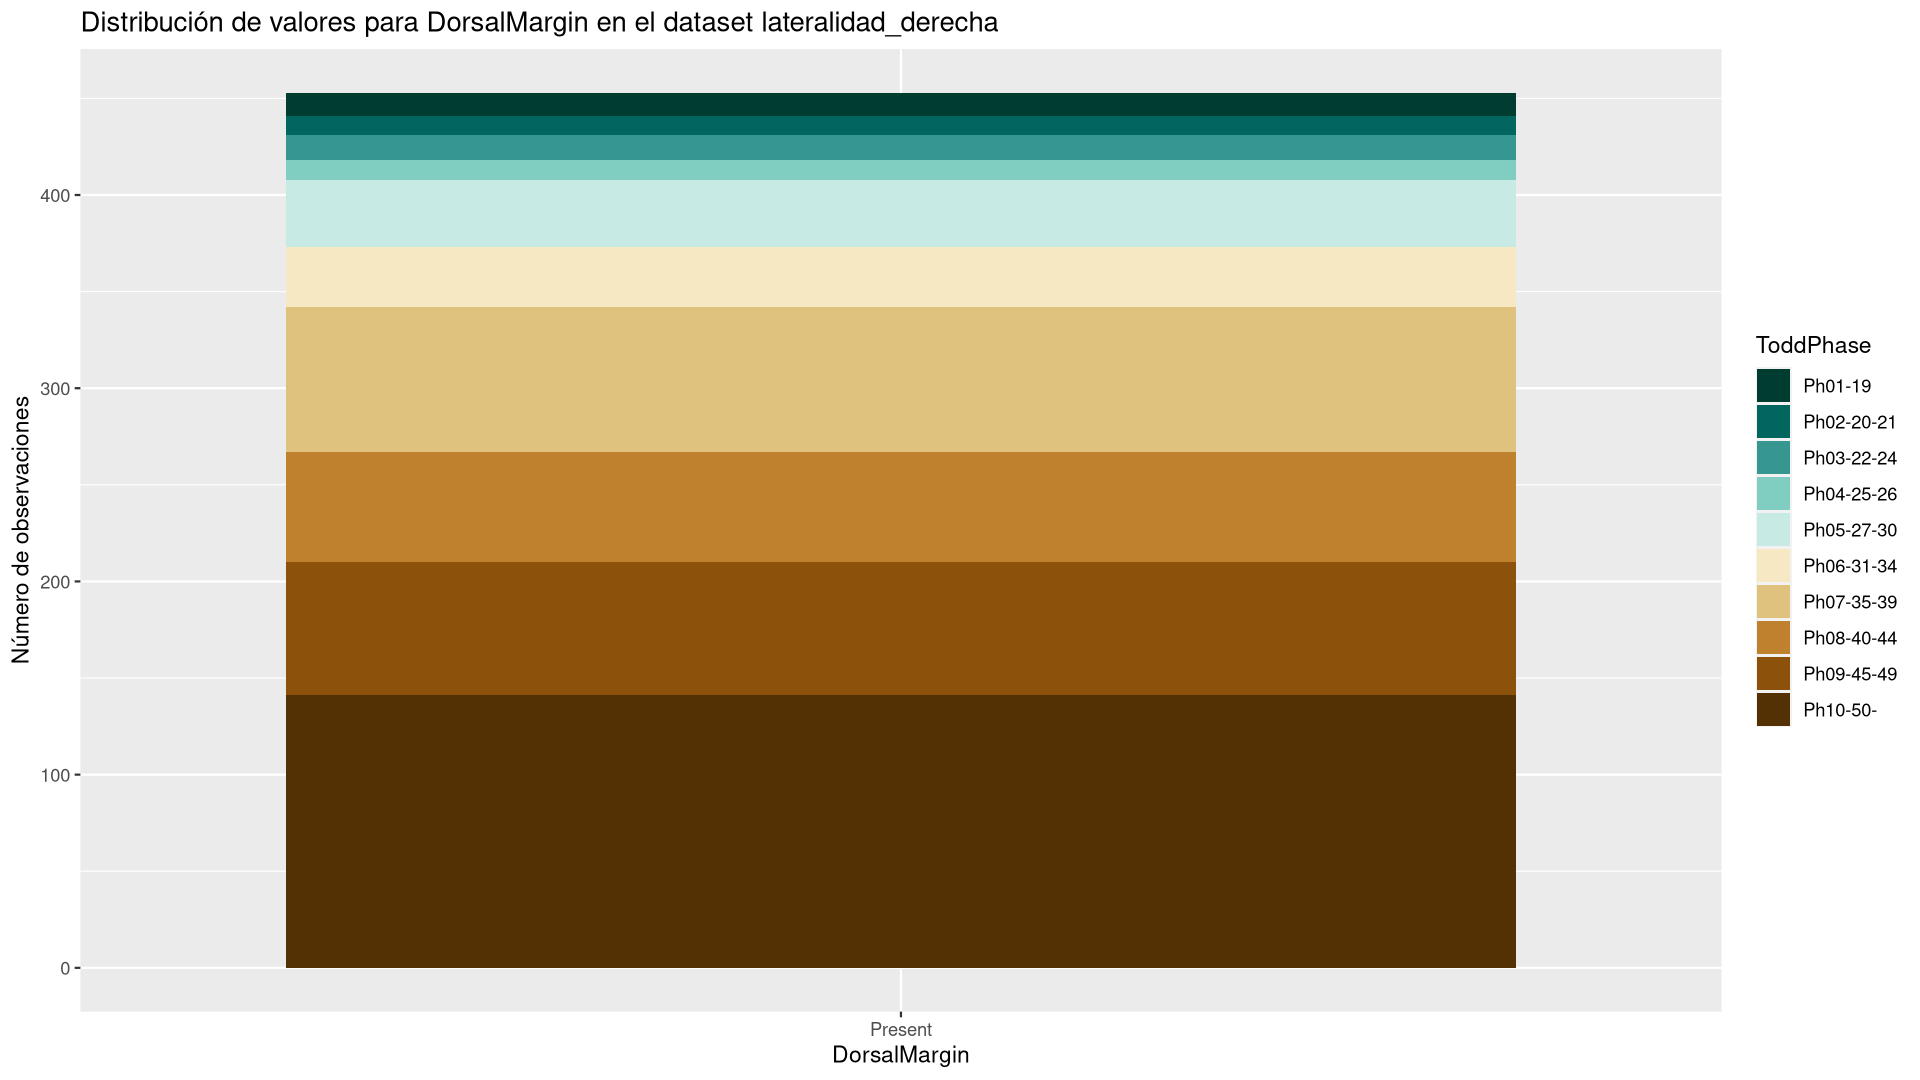
\includegraphics[width = \textwidth]{conjunto_datos/densidad_DorsalMargin_lateralidad_derecha.png}
	\caption{Distribución de los valores de DorsalMargin en el conjunto de datos de la lateralidad derecha.}
	\label{fig:densidad_DorsalMargin_derecha}
\end{figure}

\begin{figure}[H]
	\centering
	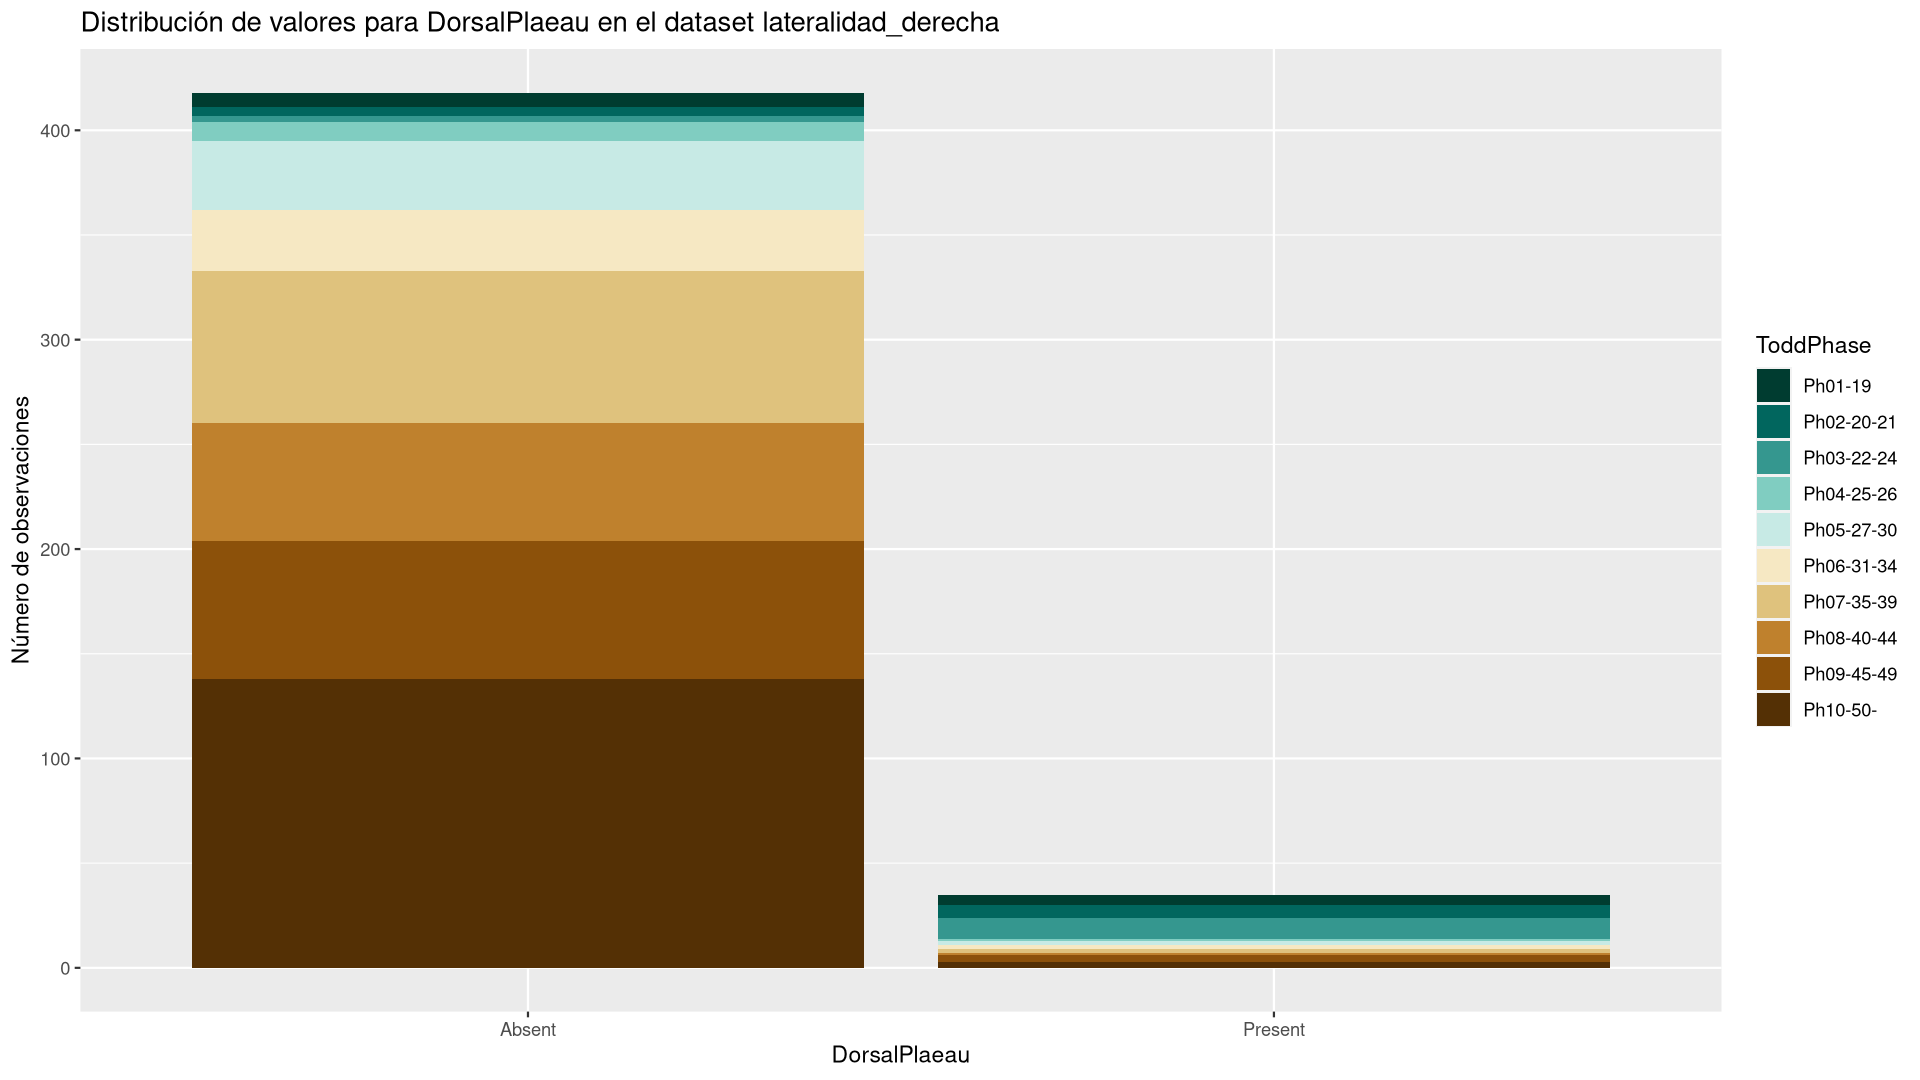
\includegraphics[width = \textwidth]{conjunto_datos/densidad_DorsalPlaeau_lateralidad_derecha.png}
	\caption{Distribución de los valores de DorsalPlaeau en el conjunto de datos de la lateralidad derecha.}
	\label{fig:densidad_DorsalPlaeau_derecha}
\end{figure}


\begin{figure}[H]
	\centering
	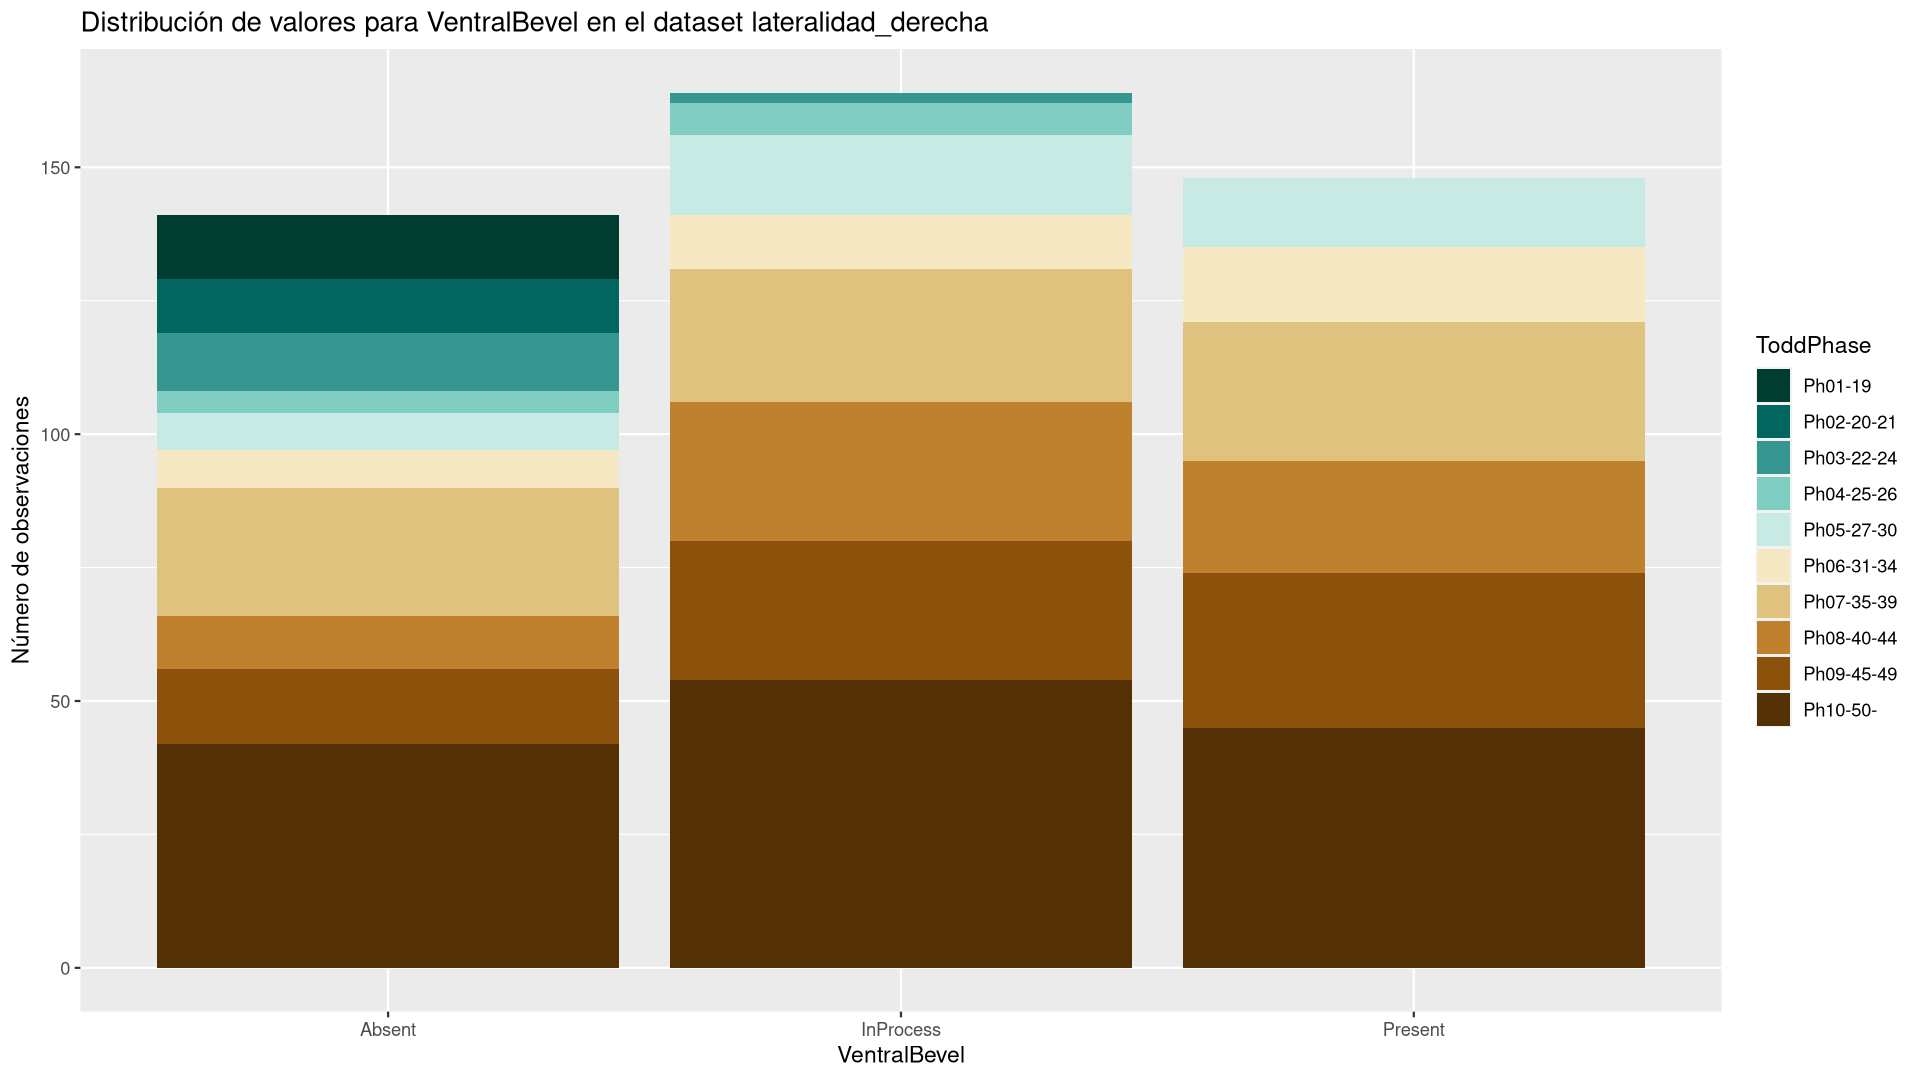
\includegraphics[width = \textwidth]{conjunto_datos/densidad_VentralBevel_lateralidad_derecha.png}
	\caption{Distribución de los valores de VentralBevel en el conjunto de datos de la lateralidad derecha.}
	\label{fig:densidad_VentralBevel_derecha}
\end{figure}

\begin{figure}[H]
	\centering
	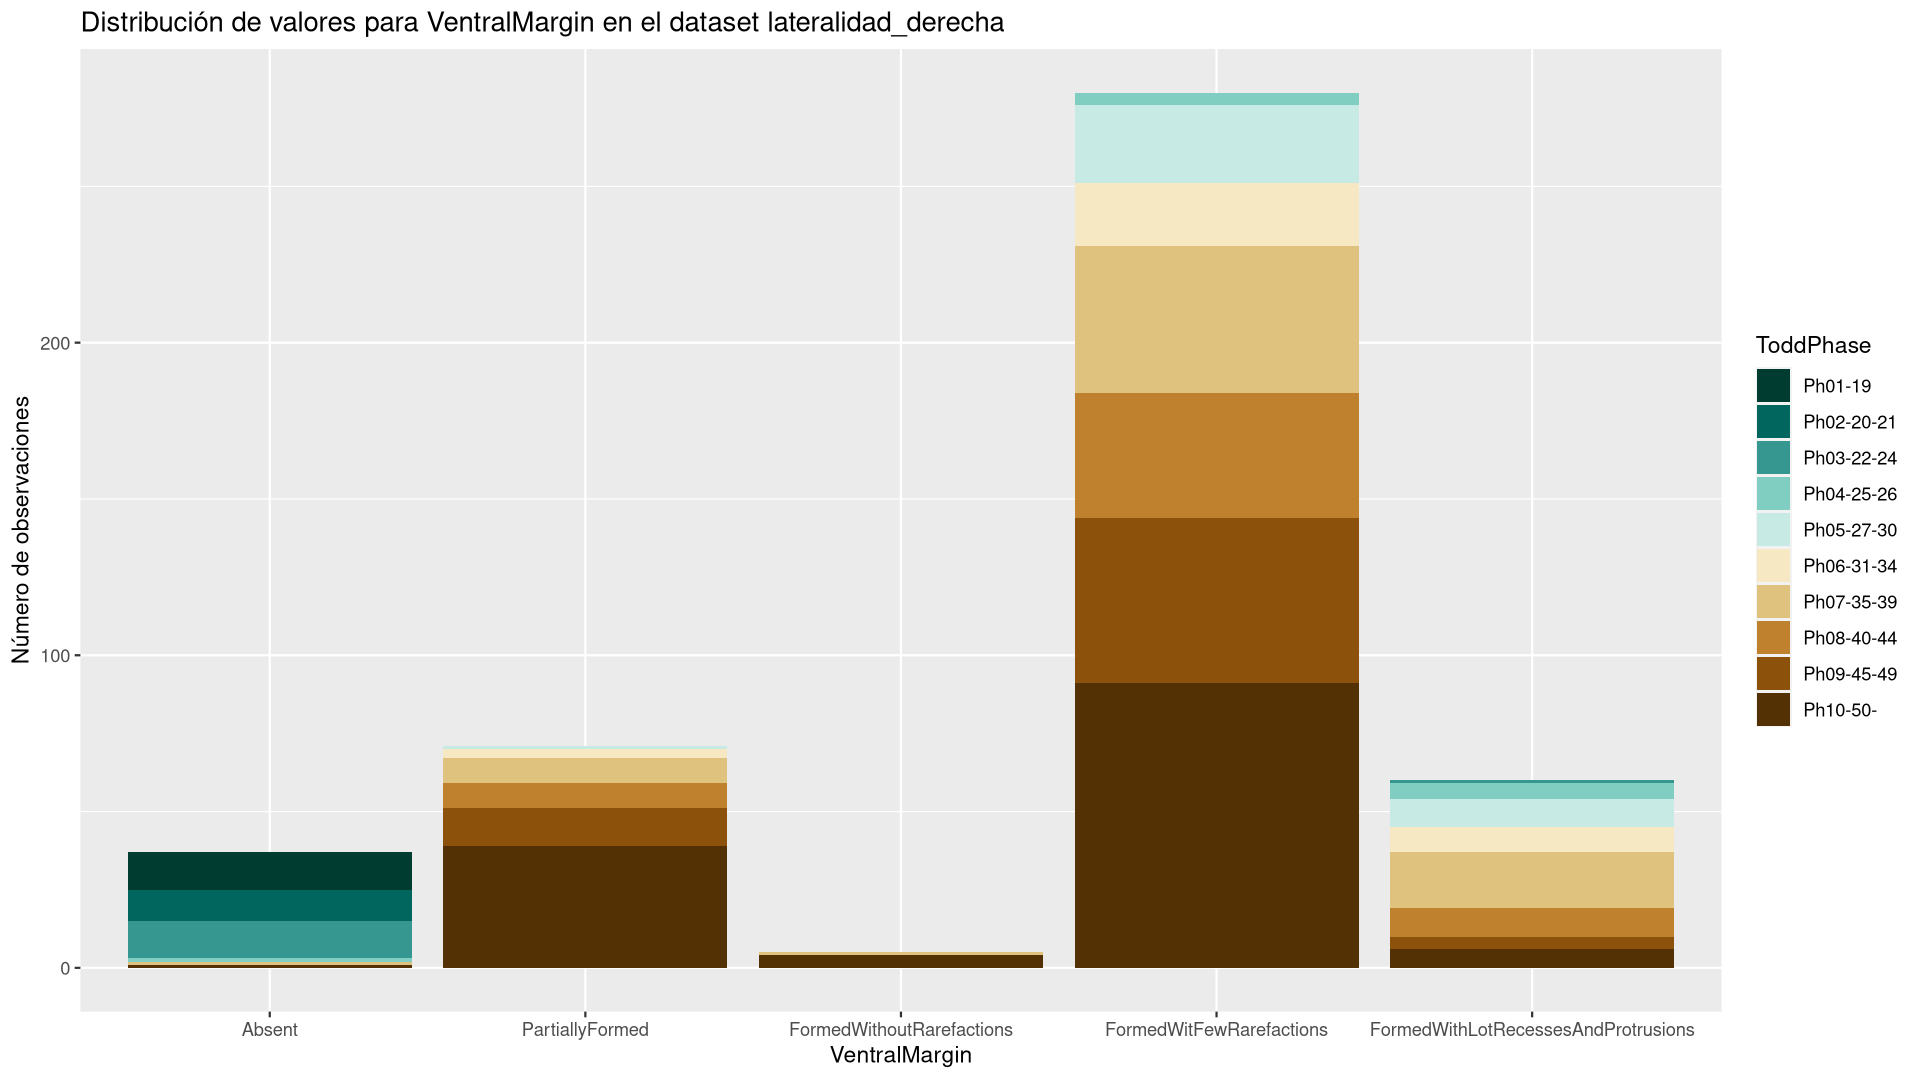
\includegraphics[width = \textwidth]{conjunto_datos/densidad_VentralMargin_lateralidad_derecha.png}
	\caption{Distribución de los valores de VentralMargin en el conjunto de datos de la lateralidad derecha.}
	\label{fig:densidad_VentralMargin_derecha}
\end{figure}

\subsubsection{Análisis del conjunto completo}

El conjunto completo de los datos cuenta con 892 observaciones, las de la lateralidad izquierda y derecha unidas. Por este motivo, al obtener las mismas conclusiones de la lateralidad izquierda y la lateralidad derecha, las conclusiones en el conjunto de datos completo cabe esperar que sean las mismas. Por este motivo simplemente vamos a comentar las más destacadas.

\begin{figure}[H]
	\centering
	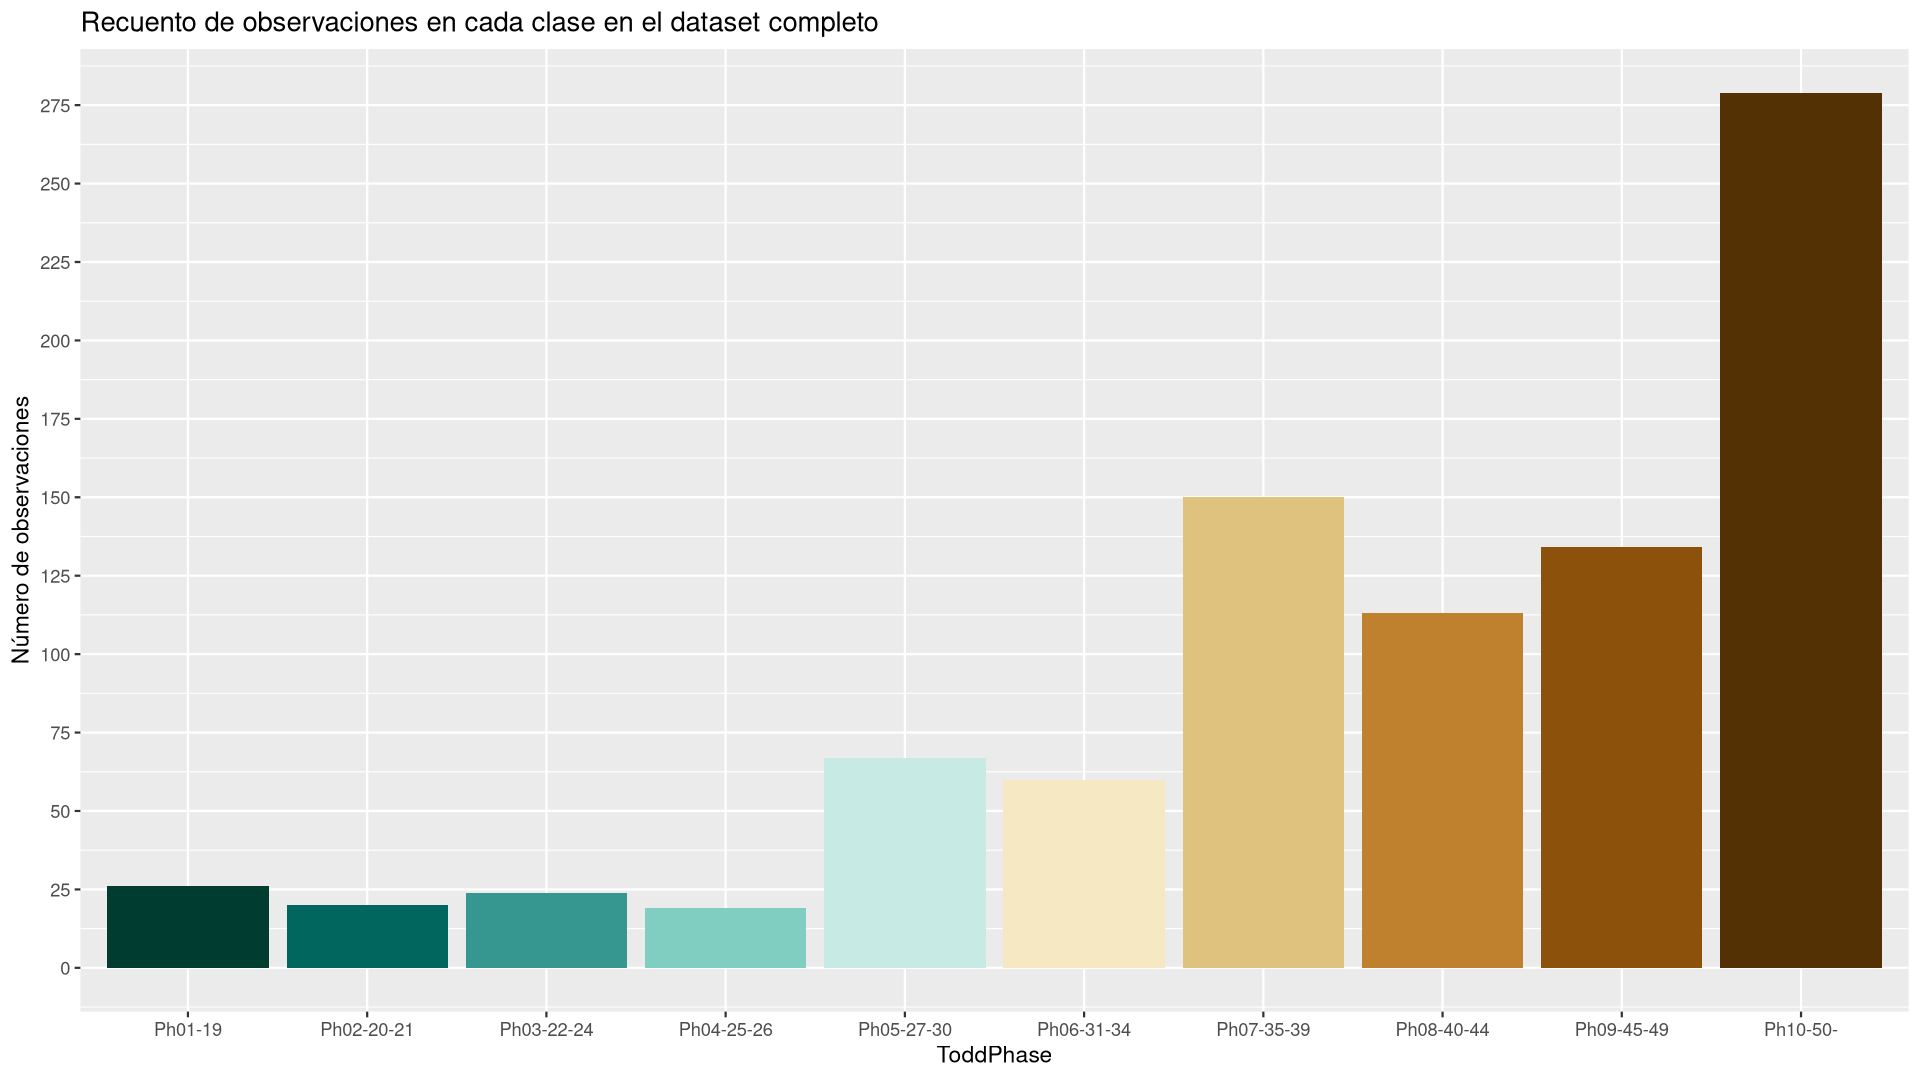
\includegraphics[width = \textwidth]{conjunto_datos/distribucion_clases_completo.png}
	\caption{Número de datos por cada fase propuesta por Todd con el conjunto de datos completo.}
	\label{fig:conteo_c}
\end{figure}


\begin{figure}[H]
	\centering
	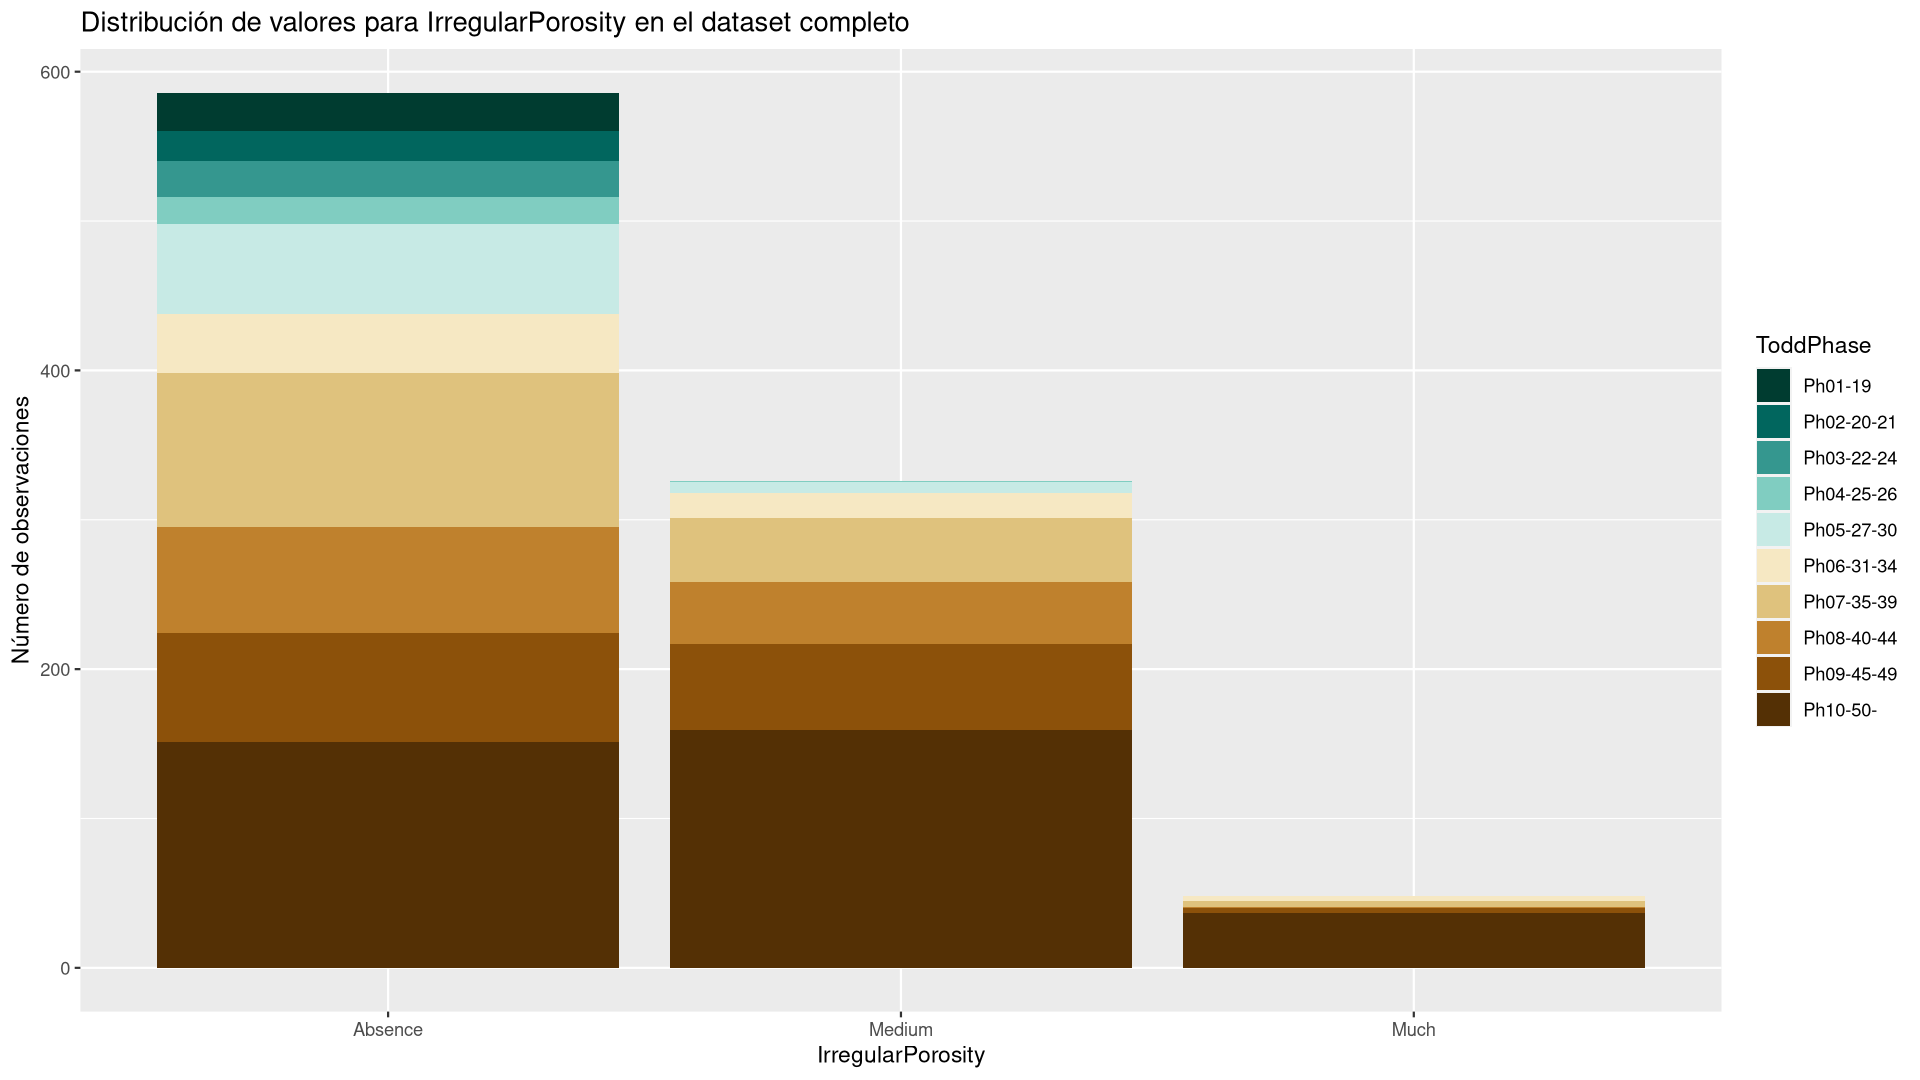
\includegraphics[width = \textwidth]{conjunto_datos/densidad_IrregularPorosity_completo.png}
	\caption{Distribución de los valores de IrregularPorosity en el conjunto de datos completo.}
	\label{fig:densidad_IrregularPorosity_completo}
\end{figure}

\begin{figure}[H]
	\centering
	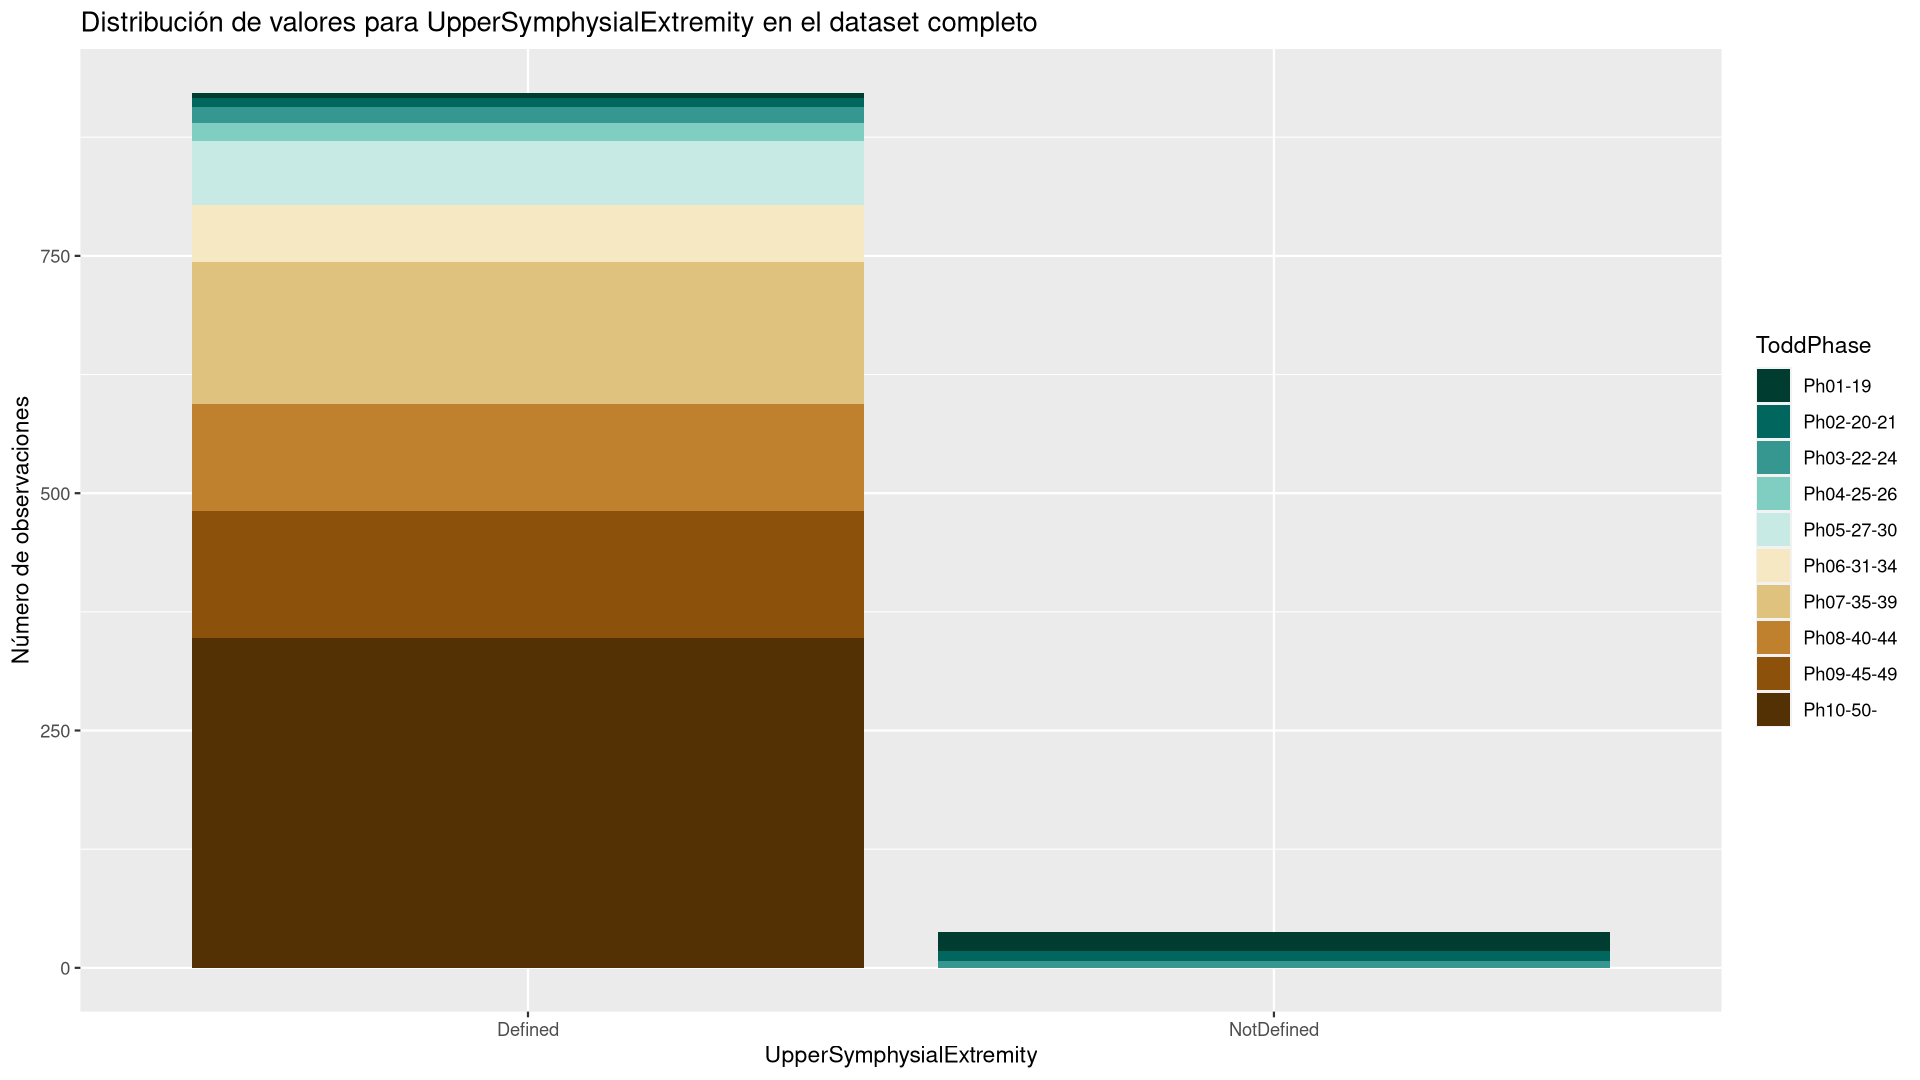
\includegraphics[width = \textwidth]{conjunto_datos/densidad_UpperSymphysialExtremity_completo.png}
	\caption{Distribución de los valores de UpperSymphysialExtremity en el conjunto de datos completo.}
	\label{fig:densidad_UpperSymphysialExtremity_completo}
\end{figure}


\begin{figure}[H]
	\centering
	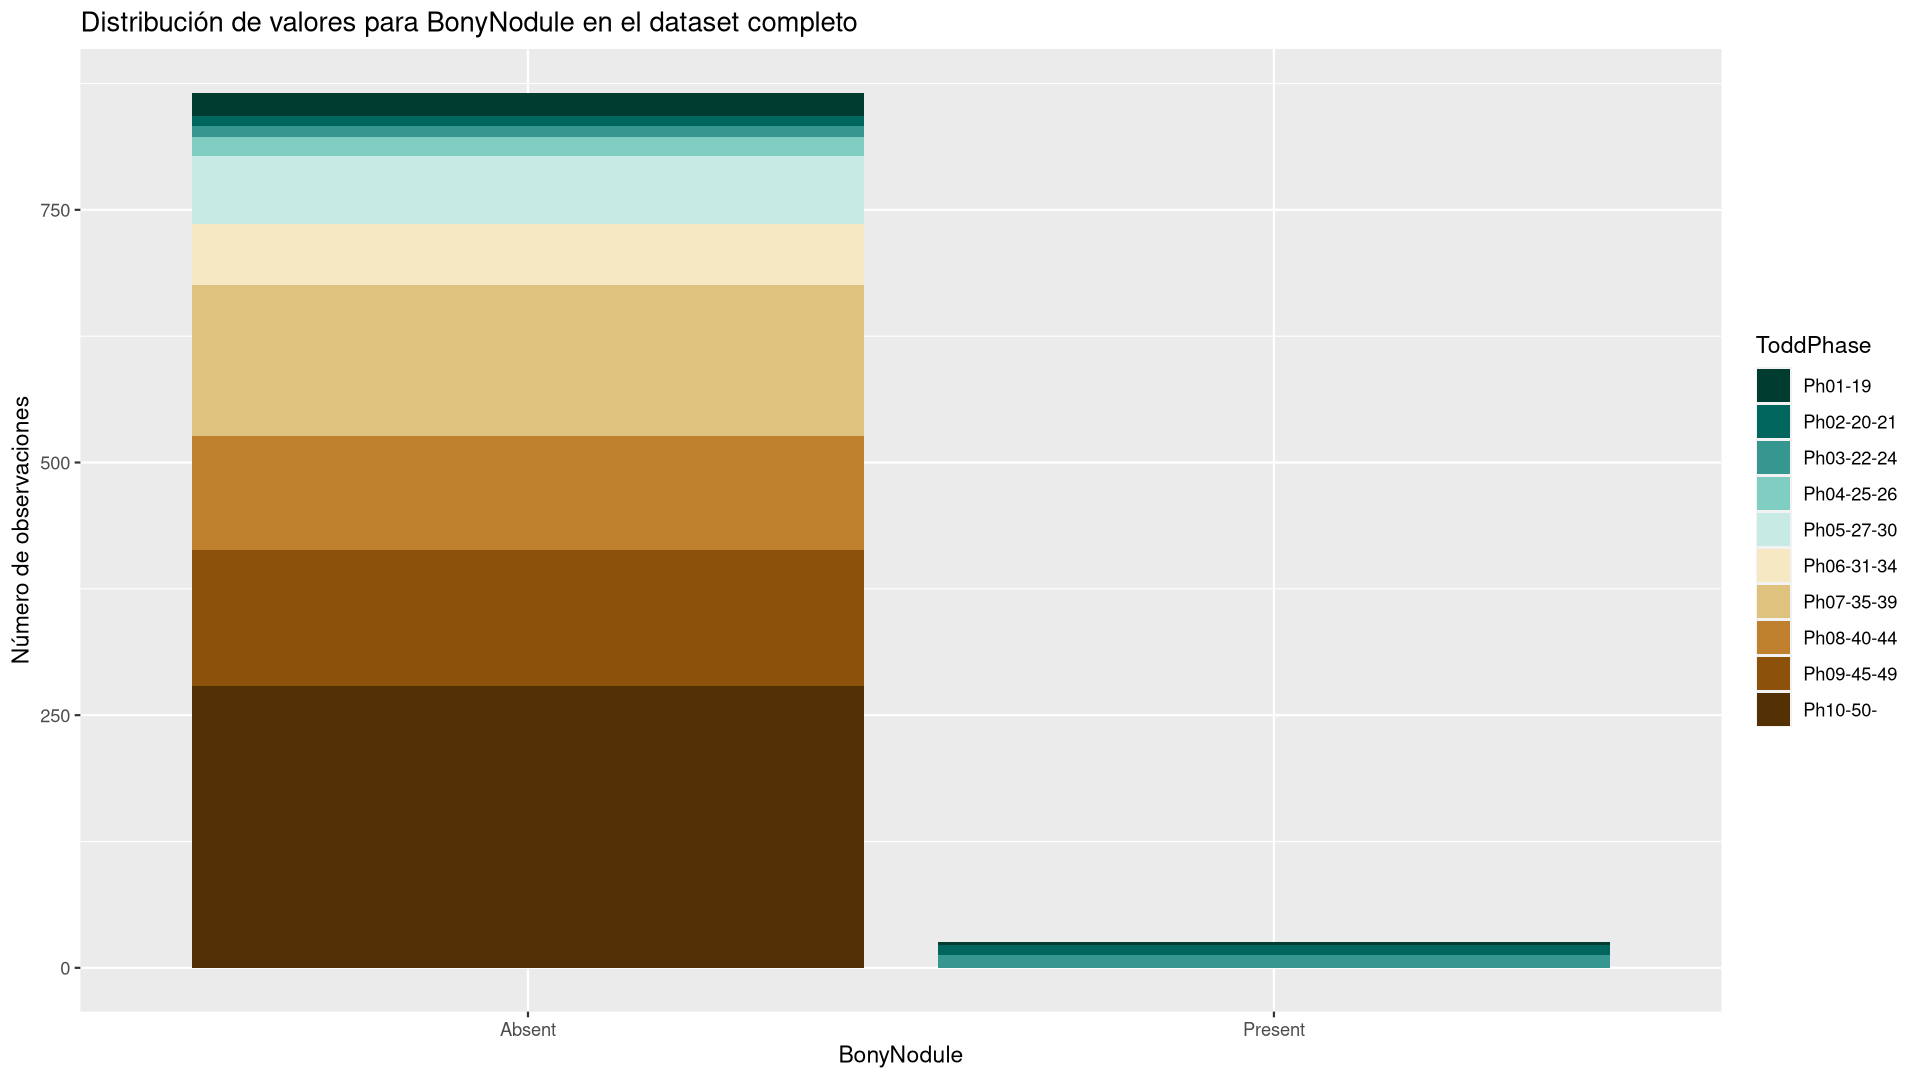
\includegraphics[width = \textwidth]{conjunto_datos/densidad_BonyNodule_completo.png}
	\caption{Distribución de los valores de BonyNodule en el conjunto de datos completo.}
	\label{fig:densidad_BonyNodule_completo}
\end{figure}



\begin{figure}[H]
	\centering
	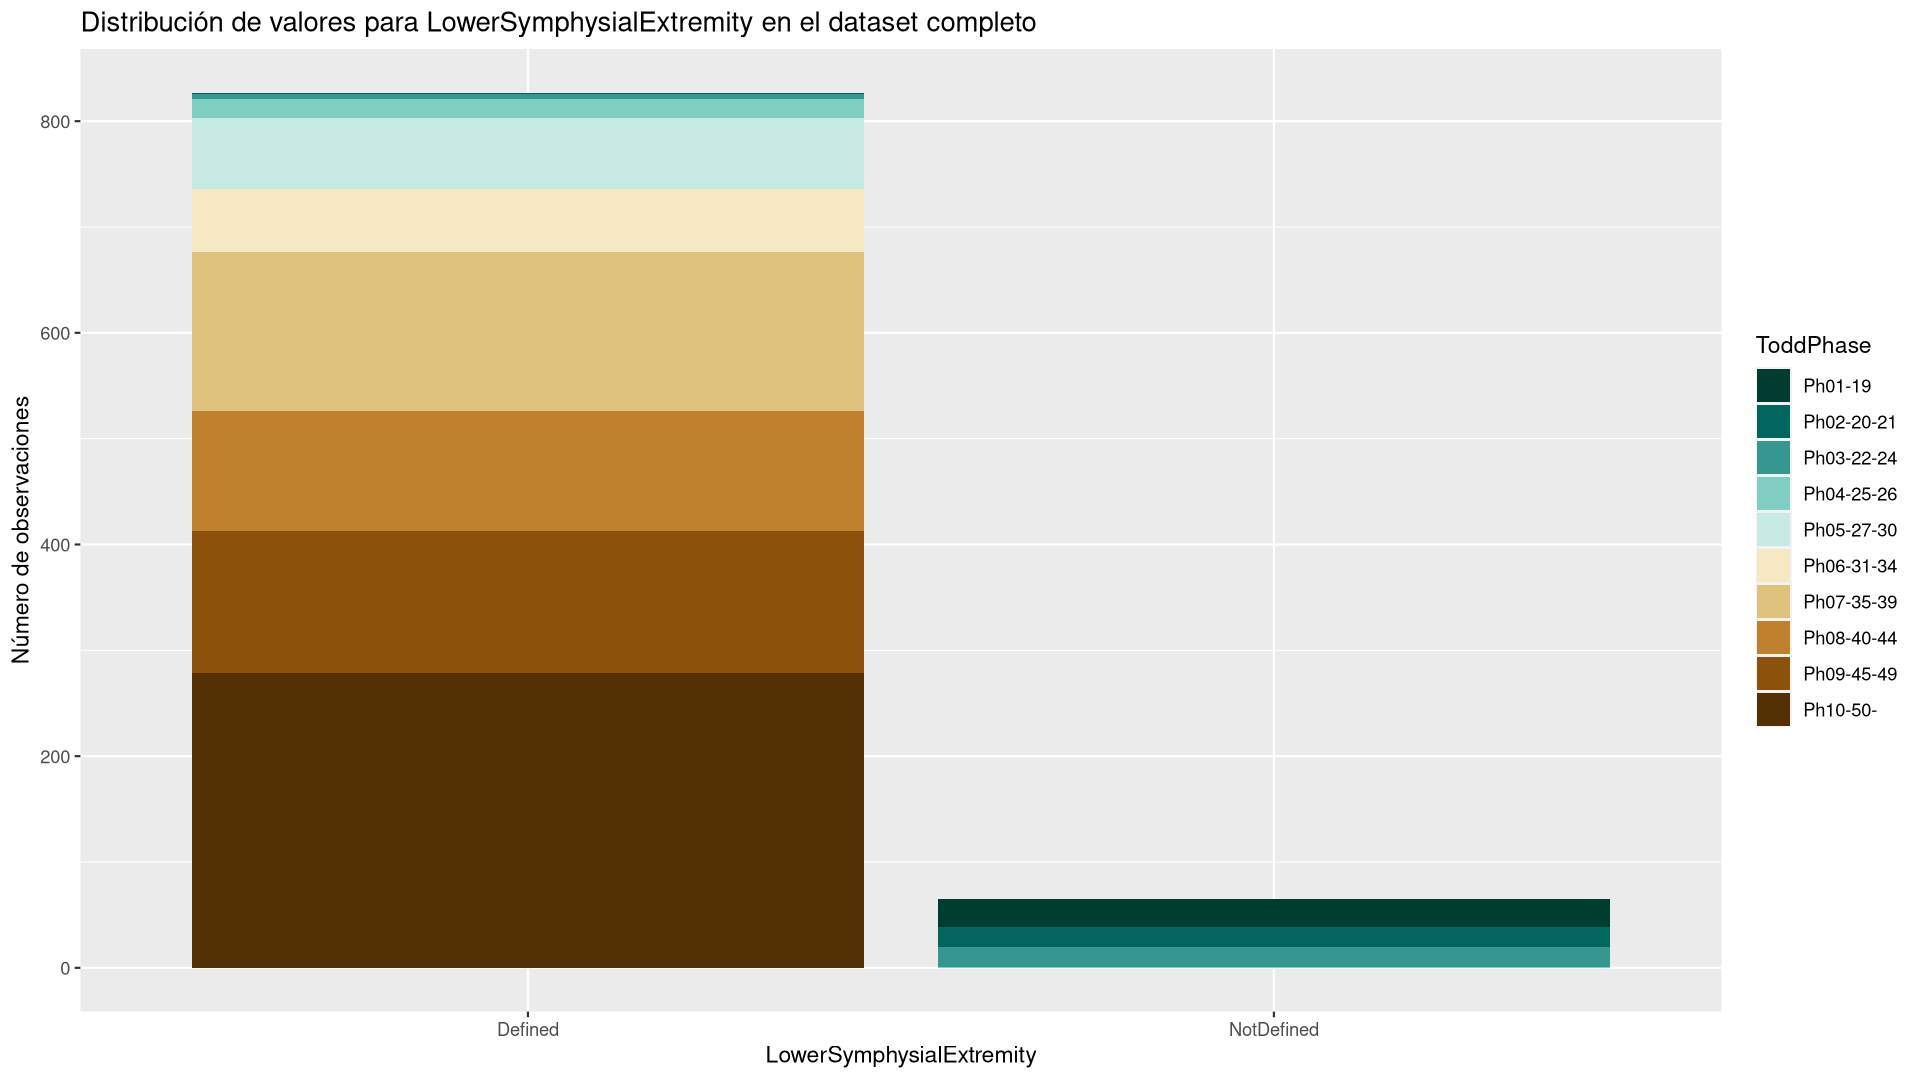
\includegraphics[width = \textwidth]{conjunto_datos/densidad_LowerSymphysialExtremity_completo.png}
	\caption{Distribución de los valores de LowerSymphysialExtremity en el conjunto de datos completo.}
	\label{fig:densidad_LowerSymphysialExtremity_completo}
\end{figure}


\begin{figure}[H]
	\centering
	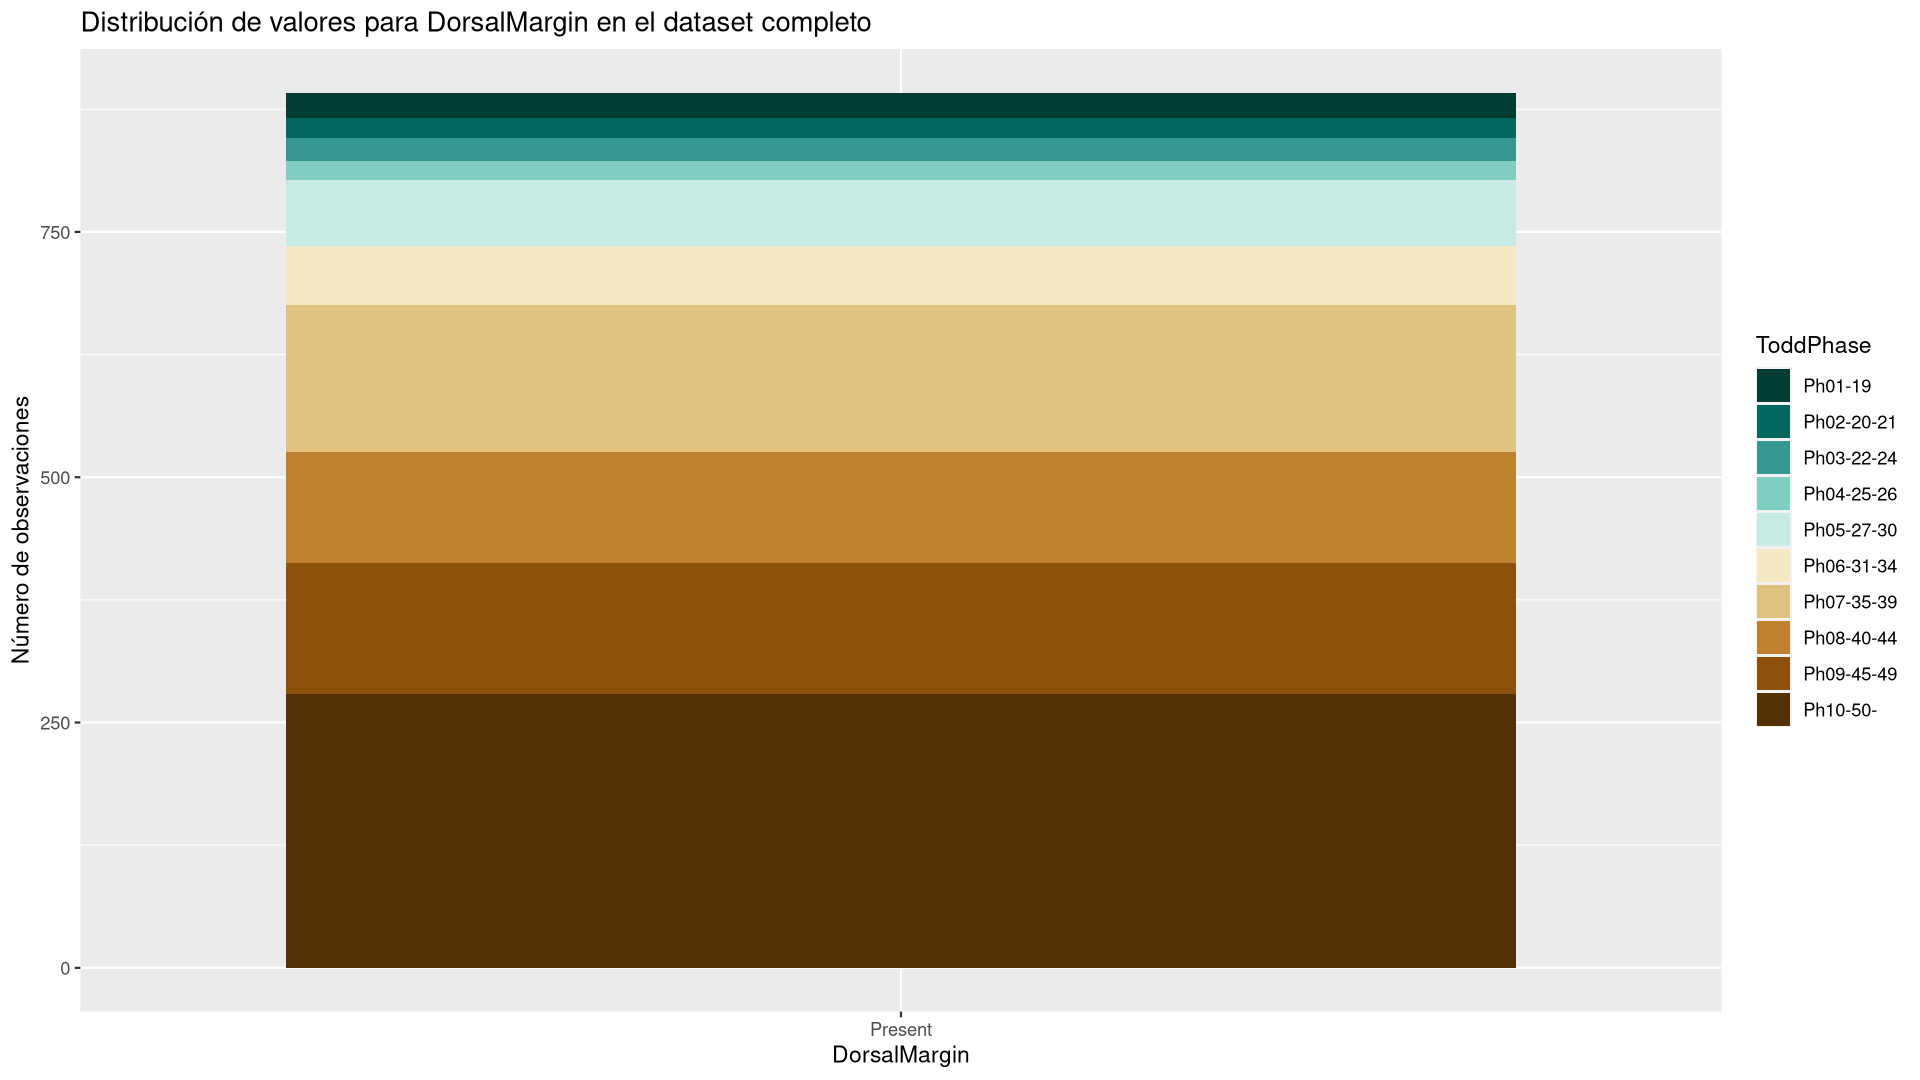
\includegraphics[width = \textwidth]{conjunto_datos/densidad_DorsalMargin_completo.png}
	\caption{Distribución de los valores de DorsalMargin en el conjunto de datos completo.}
	\label{fig:densidad_DorsalMargin_completo}
\end{figure}

En este caso cabe destacar que en todo el conjunto de datos la variable \texttt{DorsalMargin} solo toma el valor de \texttt{Present}, independientemente de la fase a la que pertenezca la observación, por lo que no aporta nada de información a la hora de realizar la clasificación y por lo tanto podemos eliminar este predictor.

\begin{figure}[H]
	\centering
	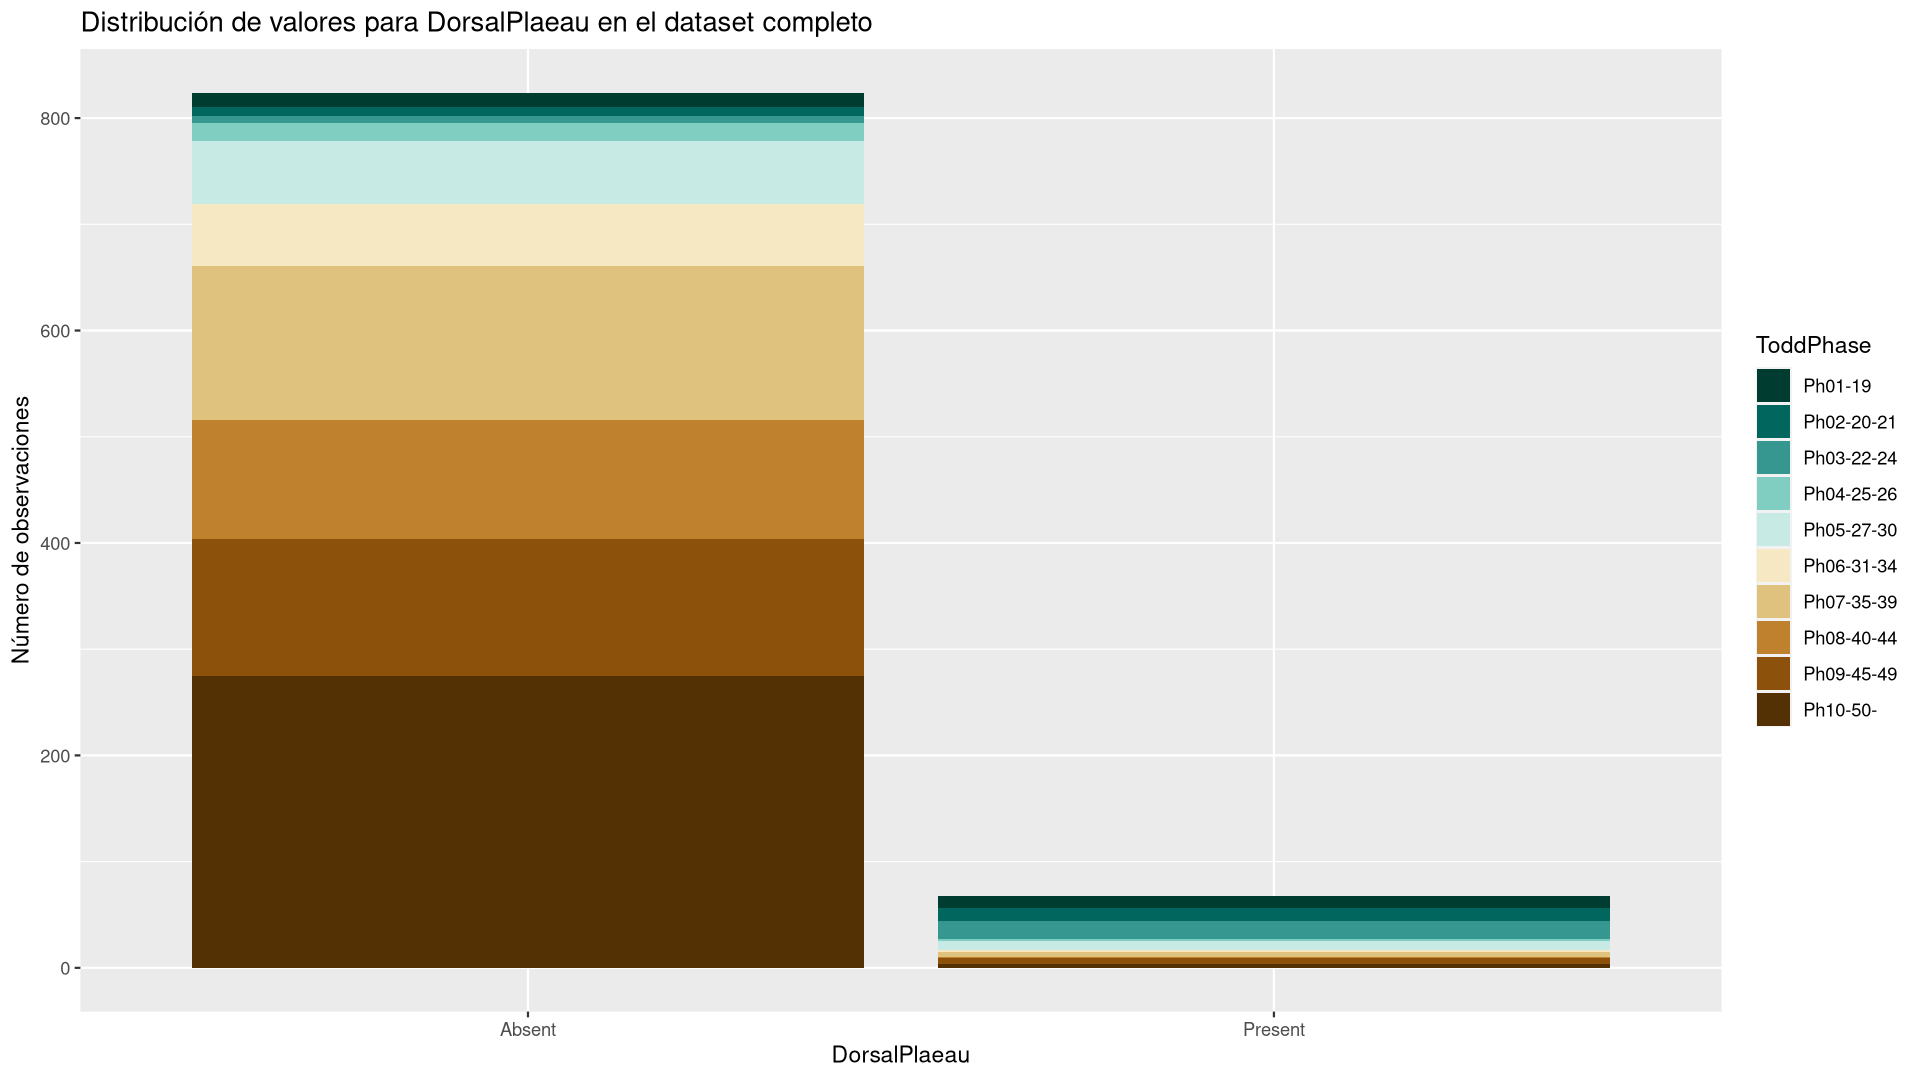
\includegraphics[width = \textwidth]{conjunto_datos/densidad_DorsalPlaeau_completo.png}
	\caption{Distribución de los valores de DorsalPlaeau en el conjunto de datos completo.}
	\label{fig:densidad_DorsalPlaeau_completo}
\end{figure}


\begin{figure}[H]
	\centering
	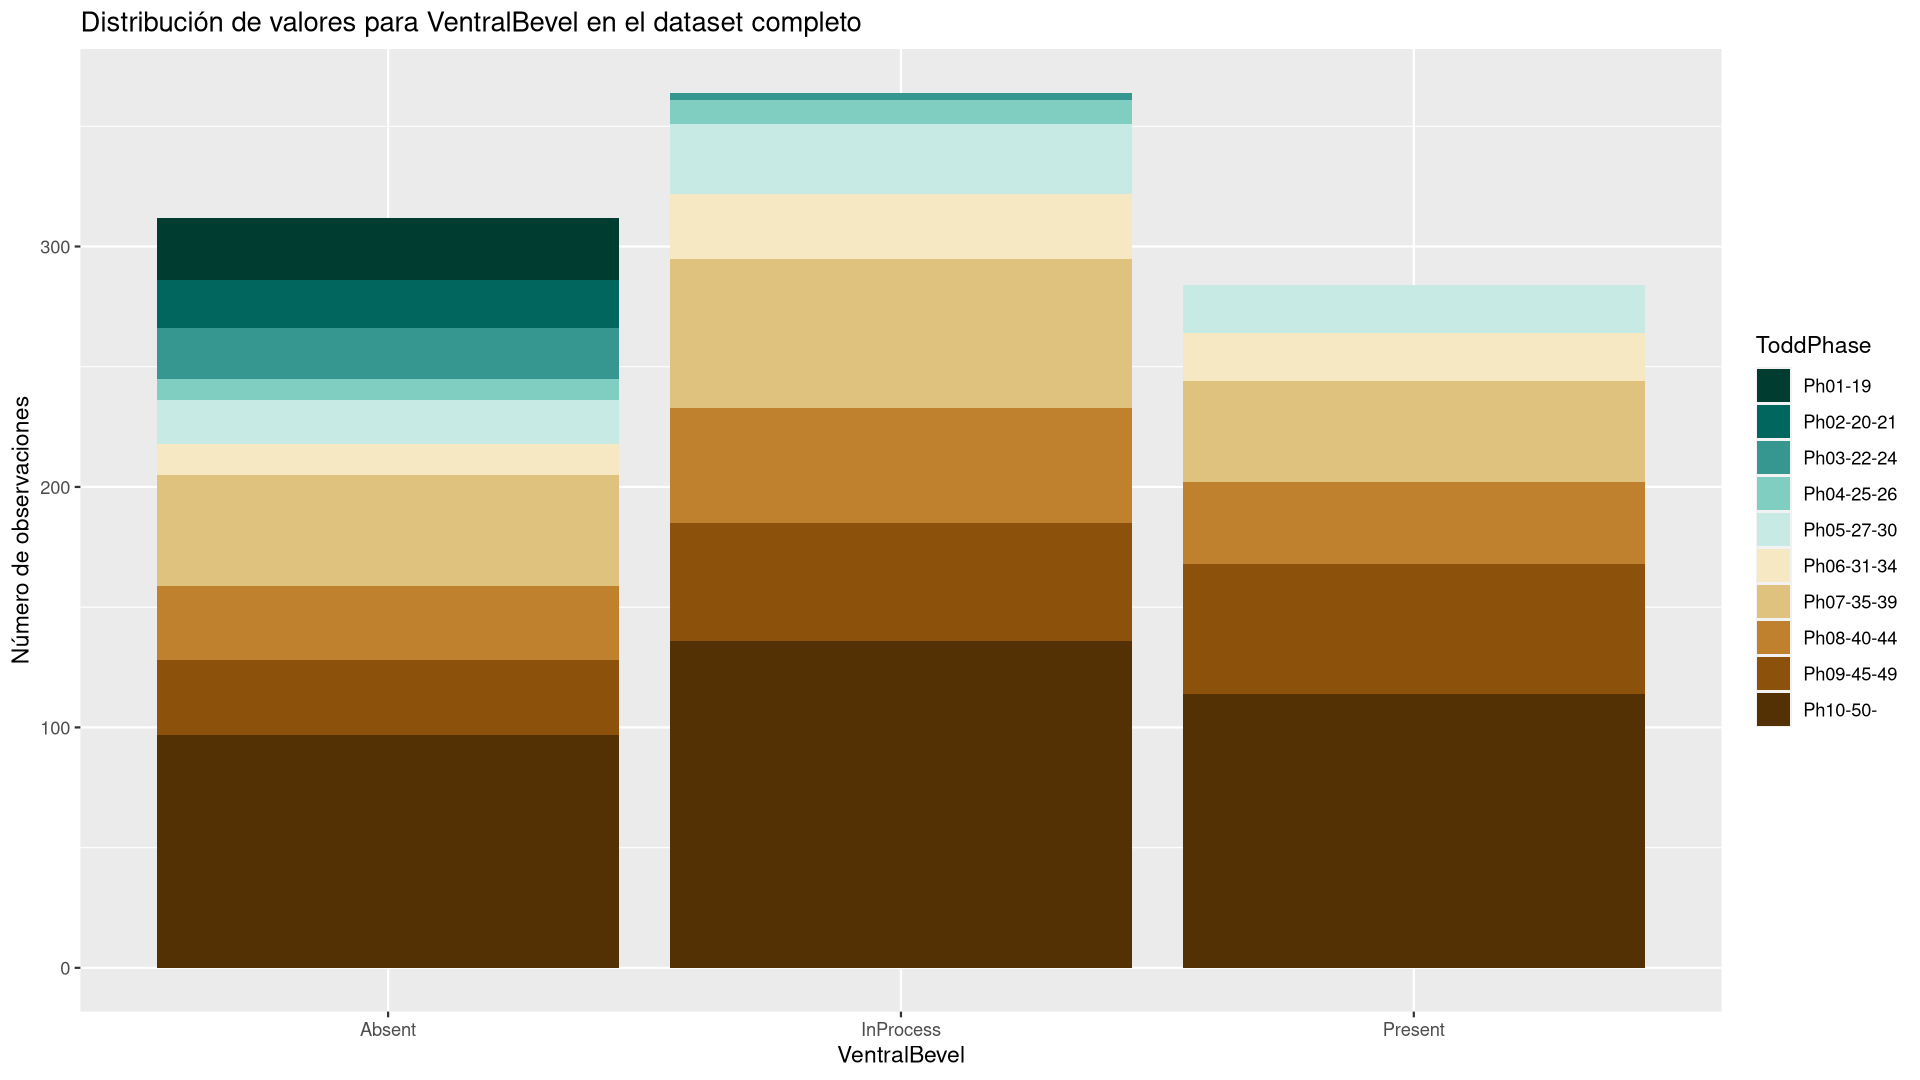
\includegraphics[width = \textwidth]{conjunto_datos/densidad_VentralBevel_completo.png}
	\caption{Distribución de los valores de VentralBevel en el conjunto de datos completo.}
	\label{fig:densidad_VentralBevel_completo}
\end{figure}

\begin{figure}[H]
	\centering
	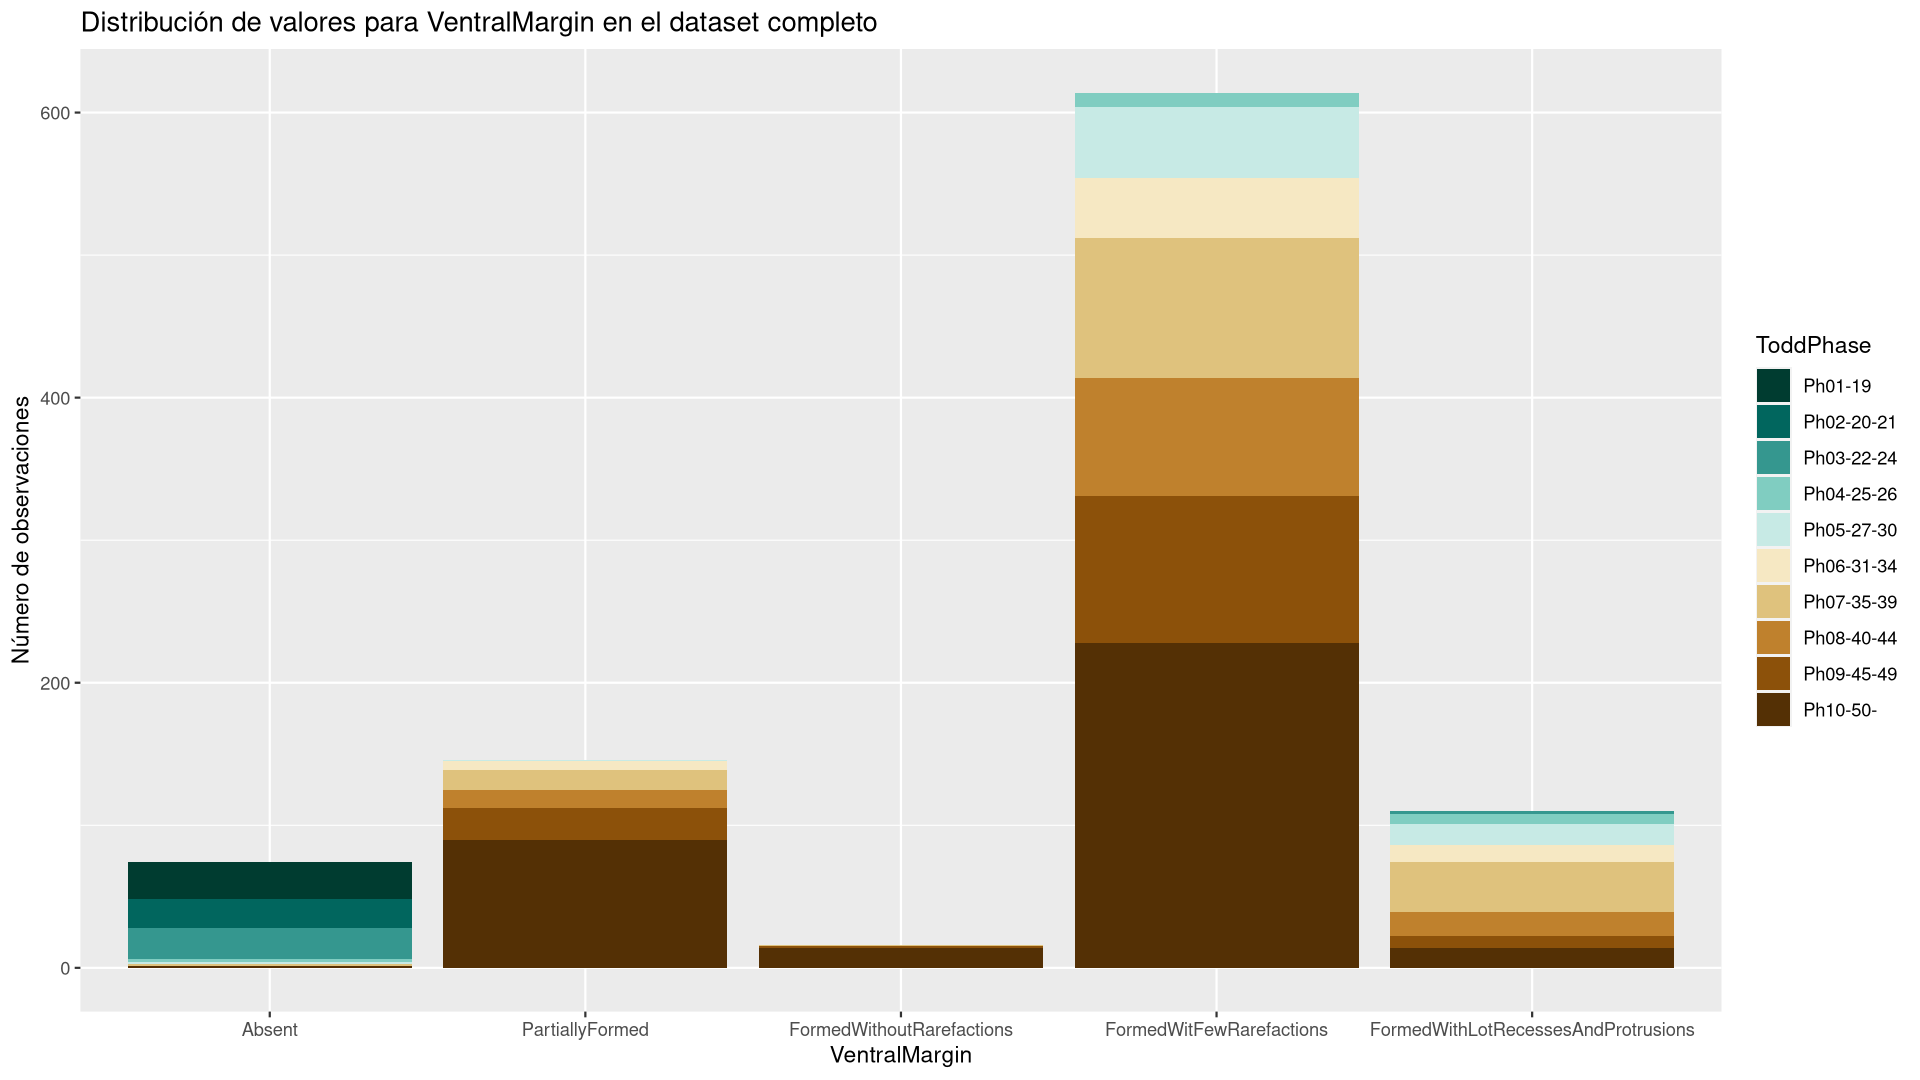
\includegraphics[width = \textwidth]{conjunto_datos/densidad_VentralMargin_completo.png}
	\caption{Distribución de los valores de VentralMargin en el conjunto de datos completo.}
	\label{fig:densidad_VentralMargin_completo}
\end{figure}

% TODO: actualizar toda la parte de sobremuestro, explicando SMOTE, borderline-SMOTE, ADASYN,
% comentar como funciona en nuestro conjunto de datos


\subsubsection{Conclusiones del análisis de datos}

Como breve resumen a este análisis de datos realizado, podemos ver como claramente este problema está desbalanceado y además es de una gran dificultad debido al gran solapamiento entre las clases, haciendo más difícil la clasificación.

También hemos podido observar distintas situaciones donde la decisión de la fase es más clara, acotando el tramo de decisión unicamente a dos o tres fases, sin embargo esto sucede con muy pocas observaciones del conjunto de datos. Hay que recordar que esto se ha hecho con un análisis univariante, es decir, observando por separado cada variable, el modelo que utilicemos tendrá a su disposición cualquier combinación de variables, con lo que se espera encontrar una mayor separabilidad entre las fases de cara a obtener un buen resultado en el problema.

Además, se ha observado que uno de los predictores, \texttt{DorsalMargin}, no aporta información al tomar únicamente un valor para todas las observaciones, independientemente de la clase, por lo que podríamos eliminar esta variable. En caso de no eliminarla, deberíamos observar que o bien no se utiliza en las reglas que obtengamos, o siempre que aparezca el valor utilizado será \texttt{Present}, que es el que siempre toma en el conjunto de datos.

Una vez realizado este análisis de datos, pasamos a las distintas técnicas de preprocesamiento que utilizaremos.


\subsection{Preprocesamiento} \label{sobremuestreo}

En esta sección se discutirá el preprocesamiento a aplicar a los datos de cara a entrenar el modelo, desde las propias transformaciones que aplicaremos a los datos, hasta si es necesario aplicar técnicas más avanzadas como sobremuestreo y reducción de ruido.

En esta sección introduciremos SMOTE y Borderline SMOTE de cara a mostrar la idea original de sobremuestreo en problemas de clasificación, su adaptación a problemas de regresión con SMOTER y finalmente una mejora de este último, SMOGN, que será el algoritmo a utilizar.

\subsubsection{Transformación de los datos}

Con respecto a las transformaciones de los datos, todo el conjunto de datos está formado por características categóricas, lo que simplificará en gran cantidad tanto la formulación de las reglas como la interpretabilidad, ya que no tendremos que manejar valores reales para las características, en cuyo caso se podría haber propuesto un sistema de reglas difuso. Por este motivo en este caso no será necesario aplicar ninguna transformación a los datos.

Si es cierto que podemos hacer una pequeña selección de características, ya que como hemos visto en el análisis inicial, en concreto en la figura \ref{fig:densidad_DorsalMargin_completo}, la característica \texttt{DorsalMargin} la podemos eliminar del conjunto de datos al no aportar información relevante, al solo tomar un valor.

Tras esto, pasamos a las propuestas para balancear el número de instancias de cada clase.

\subsubsection{Separación en conjunto de entrenamiento y test}

Tras eliminar la característica que no aportaba información, se realizará una separación de los conjuntos de datos en conjuntos de entrenamiento y de test. Esto es importante de cara a la validación del algoritmo, ya que es necesario comprobar que la propuesta se comporta adecuadamente con datos con los que no ha entrenado, aunque dentro de la propia fase de entrenamiento apliquemos una validación cruzada que se explicará más adelante.

Es importante realizar este paso antes de aplicar las técnicas de sobremuestreo para solucionar el balanceo de clases, ya que el conjunto de test no puede contener datos sintéticos, ya que se trata de una prueba real del modelo, como si fueran datos reales que nos han llegado sin etiquetar.

En este caso se ha seleccionado de forma aleatoria uniforme un 80\% de las observaciones del conjunto de datos como datos de entrenamiento y el 20\% restante como datos de test para cada conjunto de datos. Sobre este 80\% de datos serán los datos a los que apliquemos el balanceo de clases, ya que con estos datos son con los que vamos a entrenar el modelo de cara a realizar las predicciones.

\newpage

\subsubsection{Sobremuestreo: SMOTE}

SMOTE \cite{SMOTE} se trata de un método para conseguir balancear el número de datos para un problema de clasificación creando nuevos datos de las clases minoritarias de forma sintética. Fue propuesto en 2002 por varios investigadores de la Universidad de Florida del sur y la Universidad de Notre Dame.

Su funcionamiento se basa en tomar la clase minoritaria como clase positiva, y para cada elemento de dicha clase positiva buscar los $k$ vecinos más cercanos de la clase positiva. Una vez tenemos los $k$ elementos más cercanos, se crea un dato sintético entre cada vecino seleccionado y el punto original, escogiendo una zona del espacio al azar del segmento que une el vecino seleccionado y el punto original. De esta forma, modificando el número de vecinos a seleccionar, $k$, podemos ajustar el número de nuevos datos sintéticos.

\begin{figure}[H]
	\centering
	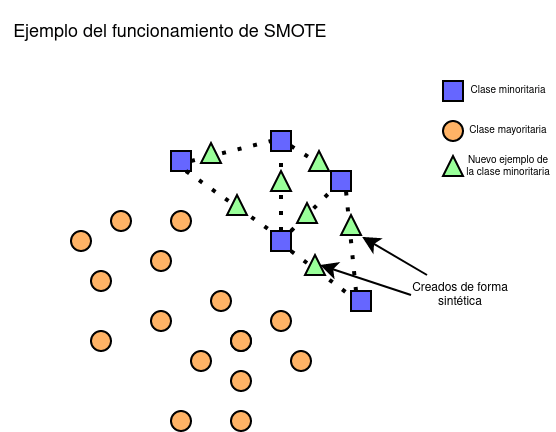
\includegraphics[scale = 0.6]{preprocesamiento/funcionamiento_smote.png}
	\caption{Ilustración de como funciona SMOTE.}
	\label{fig:funcionamiento_smote}
\end{figure}

\newpage

En su propuesta este método fue comparado con otros métodos de sobremuestreo:

\begin{figure}[H]
	\centering
	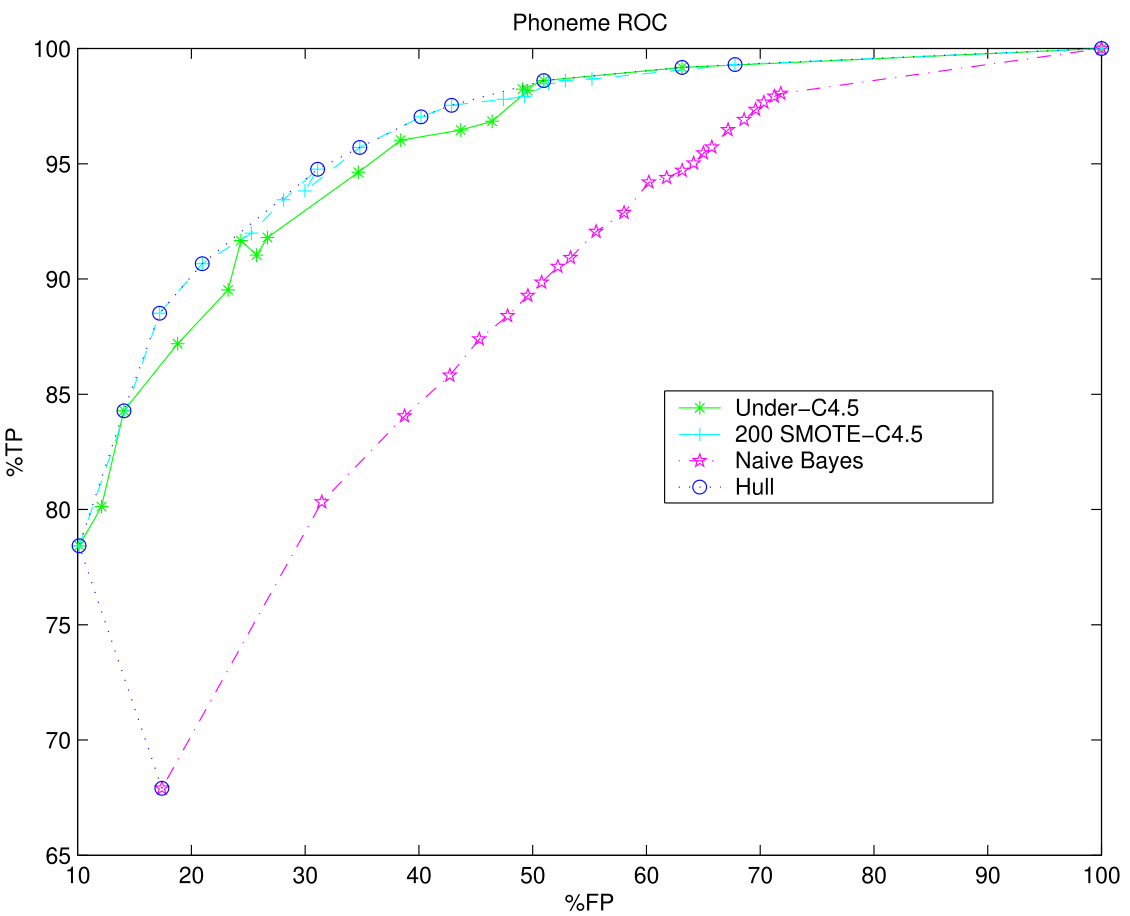
\includegraphics[scale = 1]{preprocesamiento/comparacion_ej_smote.png}
	\caption{Comparación de SMOTE con otros métodos de sobremuestreo en el conjunto de datos Phonome. En el eje X los falsos positivos y en el eje Y los verdaderos positivos. Imagen obtenida de \cite{SMOTE}.}
	\label{fig:comparacionSMOTE}
\end{figure}

Como vemos en la figura \ref{fig:comparacionSMOTE}, este método se comporta bastante bien en comparación con otros métodos y es capaz de obtener buenos resultados, sin embargo, tiene algunos problemas.

Uno de estos problemas es que cuando existe ruido entre las clases, o las clases se encuentran dispersas por el espacio de valores, gran parte de los valores sintéticos se encontrarán en una zona del espacio que no corresponde a su clase.

Este problema se hace mucho más presente en nuestro caso, al contar con tantas clases y con tantas características, y para resolverlo se propuso la variante Borderline-SMOTE.

\subsubsection{Sobremuestreo: Borderline SMOTE}

Borderline SMOTE \cite{BL-SMOTE} se trata de una variante de SMOTE que propone buscar los límites en el espacio de valores de la clase a obtener nuevos datos sintéticos, de forma que cuando se generen dichos datos nuevos, estén dentro de dichos límites. De esta forma evitamos problemas con conjuntos de datos con mucho ruido y múltiples clases.

En su artículo proponen dos variantes, una donde las nuevas muestras sintéticas son creadas a partir de todo el conjunto de datos, y otra donde las nuevas muestras solo se generan a partir de los datos considerados en el límite.


\begin{figure}[H]
    \centering
    \begin{subfigure}[b]{0.33\textwidth}
		  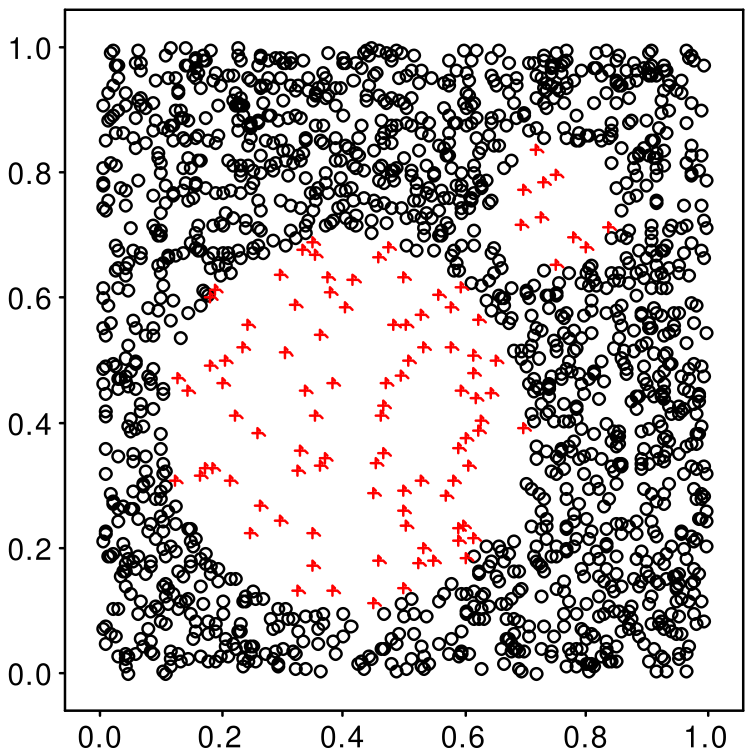
\includegraphics[width=\textwidth]{preprocesamiento/bl-smote-original.png}
        \caption{}
        \label{fig:blSMOTE-orig}
    \end{subfigure}
    \begin{subfigure}[b]{0.33\textwidth}
        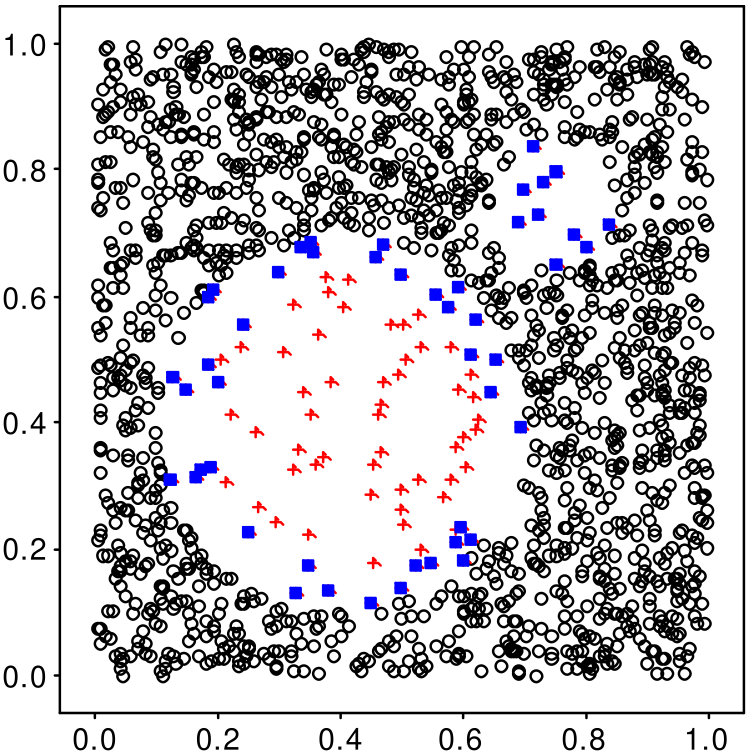
\includegraphics[width=\textwidth]{preprocesamiento/bl-smote-datos-borderline.png}
        \caption{}
        \label{fig:blSMOTE-border}
    \end{subfigure}
    \begin{subfigure}[b]{0.33\textwidth}
        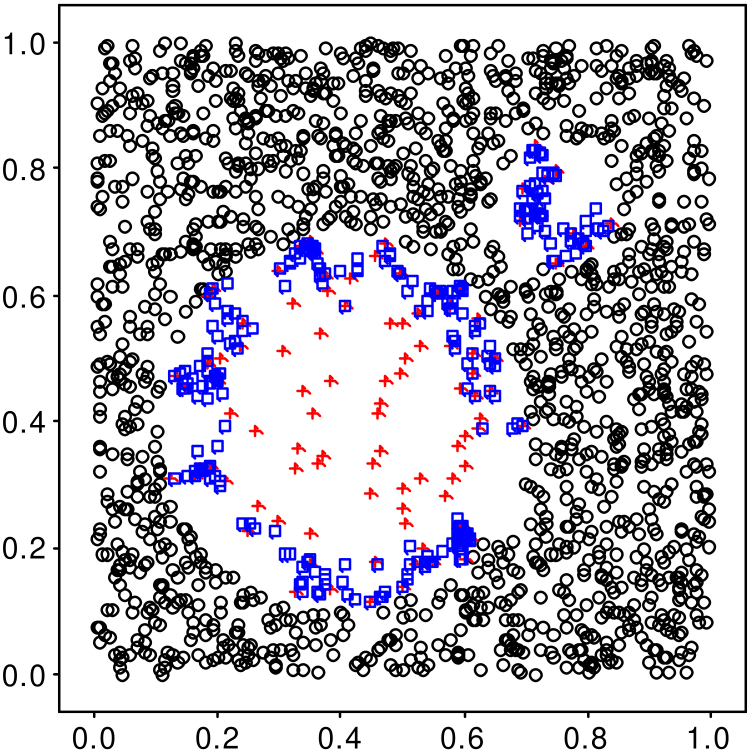
\includegraphics[width=\textwidth]{preprocesamiento/bl-smote-datos-sinteticos.png}
        \caption{}
        \label{fig:blSMOTE-sintetico}
    \end{subfigure}

    \caption{\ref{fig:blSMOTE-orig} Conjunto de datos original. \ref{fig:blSMOTE-border} datos que conforman el límite de la clase minoritaria (cuadros azules rellenos). \ref{fig:blSMOTE-sintetico} Nuevos datos generados de forma sintética dentro de los límites de la clase (cuadros azules no rellenos). Imagen obtenida de \cite{BL-SMOTE}.}
	 \label{fig:ejemploBL-SMOTE}

\end{figure}

Este método funciona de la misma forma que SMOTE a la hora de generar a los nuevos datos sintéticos, sin embargo, lo que hace es en lugar de utilizar todos los datos de la clase minoritaria, hace una preselección de datos, evitando los datos que son considerados como ruido y los datos donde es indiferente crear nuevas observaciones ya que no afectan a la frontera de decisión, es decir, se trata de una zona donde está claro que la clase es minoritaria. Esto hace que los puntos escogidos estén en la zona donde nos interesa tener datos, las fronteras entre las distintas clases, de forma que sea más facil diferenciar una clase de otra. Todo este proceso se ve ilustrado en figura \ref{fig:ejemploBL-SMOTE}.


Para comparar de forma gráfica SMOTE y BorderlineSMOTE podemos observar la siguiente ilustración utilizando datos generados de forma aleatoria con dos dimensiones:

\begin{figure}[H]
    \centering
	 \begin{subfigure}[b]{\textwidth}
		 \centering
		 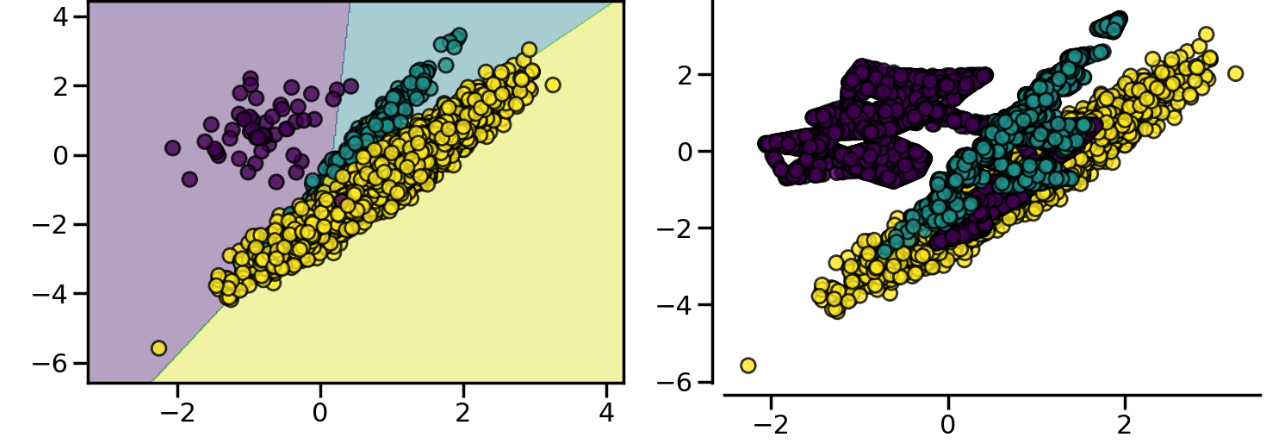
\includegraphics[width=0.8\textwidth]{preprocesamiento/resampling_smote.png}
		 \caption{A la izquierda bordes de las clases, y a la derecha sobremuestreo con SMOTE}
		 \label{fig:SMOTE-cmp}
	 \end{subfigure}

    \begin{subfigure}[b]{\textwidth}
		 \centering
		  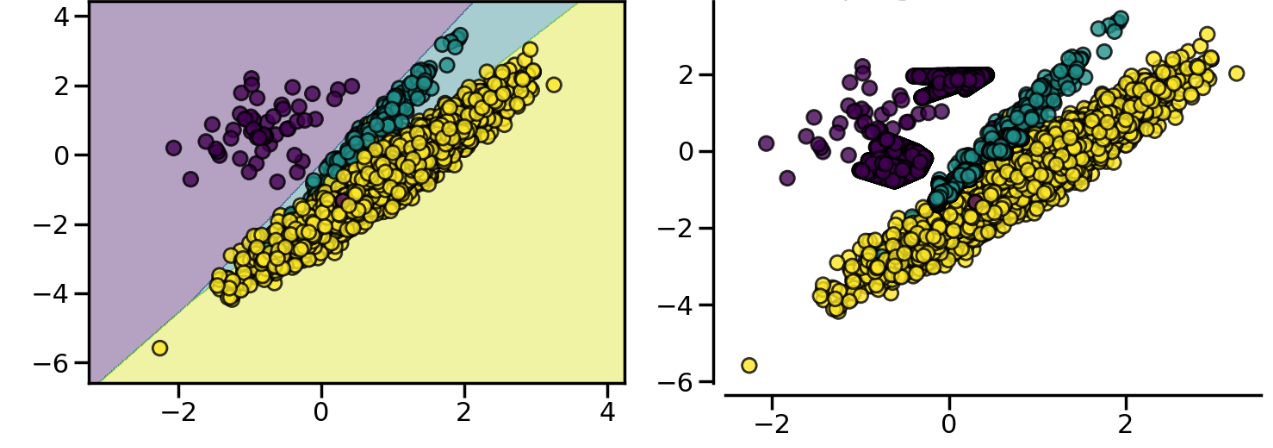
\includegraphics[width=0.8\textwidth]{preprocesamiento/resampling_blsmote.png}
        \caption{A la izquierda bordes de las clases, y a la derecha sobremuestreo con BorderlineSMOTE}
        \label{fig:BLSMOTE-cmp}
    \end{subfigure}

    \caption{Comparación de SMOTE y BorderlineSMOTE para un conjunto de datos generado aleatoriamente.}\label{fig:BLSMOTE-SMOTE}

\end{figure}

Esta claro que, como vemos en la figura \ref{fig:ejemploBL-SMOTE} y la figura \ref{fig:BLSMOTE-SMOTE}, esta técnica es mucho más versátil y conveniente que SMOTE.


\subsubsection{Sobremuestreo: ADASYN}


\subsubsection{Reducción de ruido}



\subsection{Análisis de datos tras el preprocesado}

% TODO: Ampliar esto cuando se aplique el preprocesado


\newpage
